\documentclass[10pt,twocolumn,letterpaper]{article}
\usepackage[inline]{enumitem}
\usepackage[review]{cvpr}      % To produce the REVIEW version
\usepackage{graphicx}
\usepackage{amsmath}
\usepackage{amssymb}
\usepackage{booktabs}
\usepackage[ruled,vlined]{algorithm2e}
\usepackage{epsfig}
\usepackage{physics}
\usepackage{comment}
\usepackage{subcaption}
\usepackage{framed}
\usepackage{multirow}
\usepackage{xcolor,soul}
\usepackage{latexsym,url}
\usepackage{stackengine} 

\usepackage[pagebackref,breaklinks,colorlinks]{hyperref}

\usepackage[capitalize]{cleveref}
\crefname{section}{Sec.}{Secs.}
\Crefname{section}{Section}{Sections}
\Crefname{table}{Table}{Tables}
\crefname{table}{Tab.}{Tabs.}

\def\cvprPaperID{14411} 
\def\confName{CVPR}
\def\confYear{2024}

\definecolor{todocolor}{RGB}{200,120,120}
\sethlcolor{todocolor}
\newcommand{\todo}[1]{\textcolor{black}{\hl{#1}}}

\newcommand{\multilineC}[1]{\begin{tabular}[b]{@{}c@{}}#1\end{tabular}}
\newcommand{\multilineCB}[1]{\textbf{\multilineC{#1}}}

\def\etal{{et.~al}}
\def\sota{\textsc{sota}\xspace}
\def\cnn{\textsc{cnn}\xspace}
\def\usg{\textsc{us}\xspace}
\def\gbc{\textsc{gbc}\xspace}
\def\gb{\textsc{gb}\xspace}
\def\mri{\textsc{mri}\xspace}
\def\ct{\textsc{ct}\xspace}
\def\roi{\textsc{roi}\xspace}
\def\rois{\textsc{roi}s\xspace}
\def\gbcnet{\textsc{gbcn}et\xspace}
\def\mssop{\textsc{MS-SOP}\xspace}
\def\myarch{FocusMAE\xspace}

\newcommand{\myfirstpara}[1]{\noindent \textbf{#1.}}
\newcommand{\mypara}[1]{\vspace{0.1em} \myfirstpara{#1}}

\newcommand\oast{\stackMath\mathbin{\stackinset{c}{0ex}{c}{0ex}{\ast}{\bigcirc}}}

\newcommand{\beginsupplement}{%
        \setcounter{table}{0}
        \renewcommand{\thetable}{S\arabic{table}}%
        \setcounter{figure}{0}
        \renewcommand{\thefigure}{S\arabic{figure}}%
     }

\begin{document}

\title{FocusMAE: Gallbladder Cancer Detection from Ultrasound Videos with \\ Focused Masked Autoencoders}

\maketitle

%\doublespacing
\onehalfspacing
\pagestyle{plain}
\addcontentsline{toc}{chapter}{Abstract}
\chapter*{Abstract}

Gallbladder Cancer (GBC) is the most common biliary tract cancer and the 5th most common gastrointestinal tract malignancy. India sees about 20\% of annual GBC-related deaths worldwide and faces an incidence rate compared to the global highest. The overall mean survival rate for patients with advanced GBC is only six months, and the 5-year survival rate is less than 5\%. Early diagnosis and curative surgical resection remain the only hope to improve the bleak survival statistics. Ultrasound (USG) is a popular and excellent candidate diagnostic modality for abdominal ailments in low-resource settings due to its low cost, availability, and ionizing radiation-free nature. USG is also the first-line diagnostic modality for gallbladder (GB) diseases. However, diagnosing GBC in USG is difficult, even for experienced radiologists, due to the overlapping visual features of benign and malignant GBs and various confounding medical conditions such as cholecystitis, pancreatitis, and Rokitansky-Aschoff sinuses. Our experiments reveal that human experts could achieve only about 70\% sensitivity (recall) in differentiating GBC from benign diseases (dichotomous classification) from USG. 

\par Inspired by the recent success and the transformational capabilities shown by Machine Learning (ML) models, especially the Deep Neural Networks (DNNs), in a plethora of medical image computing tasks, we investigate leveraging DNNs to detect GBC from USG. However, the low image quality arising from noise and artifacts such as shadows or textures, the operator bias and variation in view due to handheld sensors, and the lack of annotated data make the application of DNNs difficult in USG. 

\par In our pursuit of enhancing diagnostic capabilities, we systematically explore the potential of deep convolutional models, leading to the development of GBCNet. GBCNet is a two-stage DNN that first localizes the GB or the region-of-interest (ROI), and then employs a specialized classifier based on multi-scale, second-order pooling (MS-SoP) for robust GBC detection. We further develop a Gaussian smoothing-based training curriculum inspired by human visual acuity to mitigate the effect of spurious textures. GBCNet tackles issues such as noise, artifacts, and viewpoint variation in USG imaging, improving the GBC detection sensitivity by 7 points compared to SOTA DNN models and 20 points compared to expert radiologists. 

\par The reliance on bounding box annotations for training GBCNet's localization component presents a significant bottleneck, given the high cost and complexity of obtaining such annotations. To overcome this challenge, we utilize limited supervised data by introducing -- (1) an unsupervised contrastive framework for learning GBC representations from unlabelled videos, and (2) a weakly supervised object detection technique to use only image labels instead of bounding box annotation requirements, thus designing more practical models for real-world deployment. 

\par We address the crucial aspect of interpretability in GBC detection by introducing RadFormer, a deep neural network architecture capable of generating interpretable explanations for its decisions. RadFormer not only improves detection sensitivity over GBCNet but also aids in understanding the underlying visual features relevant to GBC diagnosis, bridging the gap between AI-based detection and clinical interpretability. 

\par Finally, we advocate for a paradigm shift towards video-based GBC detection, leveraging the rich spatiotemporal information available in full USG videos. Video-based detection is also clinically more relevant as single frames may not contain conclusive evidence for disease detection. We introduce an innovative masked auto-encoder design called FocusMAE, to learn self-supervised representations for GBC from USG videos. We demonstrate significant improvements in GBC detection using FocusMAE, achieving a 100\% sensitivity and thus showcasing the potential of video-based approaches in streamlining the detection process and reducing operator-specific variations.

\par In summary, we designed and developed accurate, data-efficient, interpretable, and clinically relevant DNN models which could overcome the challenges such as noise, artifacts, viewpoint variability, data scarcity, and real-time applicability in detecting GBC from USG, thereby opening future avenues for transformational research.

% Gallbladder Cancer (GBC) is the most common biliary tract cancer and the 5th most common gastrointestinal tract malignancy. India sees about 20\% of annual GBC-related deaths worldwide and faces an incidence rate compared to the global highest. The overall mean survival rate for patients with advanced GBC is only six months. Early diagnosis and curative resection remain the only hope to improve the outcomes. Ultrasound Sonography (USG) is a popular and excellent candidate diagnostic modality for abdominal ailments in low-resource countries. However, the clinical characterization of GBC in USG is difficult, even for experienced radiologists. The low image quality due to noise and artifacts, and the variation in view due to handheld sensors, make automated detection difficult. In this work, we investigate leveraging Deep Neural Networks (DNNs) to detect GBC from USG and tackle the challenges posed by USG. 

% We first address inherent issues in ultrasound images — noise, shadows, and spurious textures- and develop a robust model (GBCNet) to improve the accuracy of predictions significantly. Our focus then extends to improving interpretability in model decisions, introducing RadFormer to provide insights behind predictions, and enhancing its practicality in clinical settings. Additionally, we explore a pivotal challenge in medical computer vision — learning from limited supervised data and developing a self-supervised contrastive pretraining framework. We also leverage the USG video data to build a robust model for GBC detection in videos, eliminating the manual frame selection by radiologists and streamlining the entire detection process.


\section{Introduction}

%\myfirstpara{Gallbladder Cancer (GBC)}
%
%Lately, automated GBC detection has drawn an increased interest from the researchers \cite{basu2022surpassing, basu2023radformer, chang2022ct, kinoshita2023deep}. GBC is difficult to detect at an early stage \cite{howlader2017seer}, and surgical resection becomes infeasible for most patients as the disease gets detected at a late stage. As a result, the disease shows bleak survival statistics. The 5-year survival rate for patients with advanced GBC is only 5\%, and the mean survival time is six months \cite{randi2006gallbladder, gupta2021locally}. Hence, early detection of GBC is crucial for timely intervention and improving the survival rate \cite{hong2014surgical}. %Earlier studies suggest that early detection of GBC can improve the 5-year survival rate significantly \cite{hong2014surgical}.

%\mypara{Ultrasound (USG) for GBC Detection}
%
%USG has been the preferred non-invasive diagnostic imaging modality owing to its low cost, accessibility, and non-ionization. Often, it is the sole imaging performed on patients with abdominal diseases in low-resource countries. However, unlike benign afflictions like stone or polyp, identifying signs of malignancy from routine USG is challenging for radiologists \cite{gupta2020imaging,gb-rads-paper}. GBC may advance silently if it remains undetected. Thus, it is imperative to identify GBC from USG at an early stage. 

\mypara{Motivation}
%
%Detecting GBC from USG images using Deep Neural Networks (DNNs) is challenging. As we have discussed in \Cref{chap:usg}, USG images often have low quality due to sensor issues such as shadows or textures, causing biases in DNNs and making it hard to pinpoint the gallbladder (GB) region accurately. The handheld nature of the probe also means the views are not aligned, adding to the challenge. Malignant cases, unlike the non-malignant one, may not demonstrate clear anatomy due to the presence of lesions. GBC is also difficult to detect due confounding medical conditions. 
Our earlier efforts to circumvent the challenges (earlier discussed in \Cref{sec:challenges}) of USG for accurate GBC detection techniques are primarily image-based. 
Image-centric methodologies demonstrate shortcomings in capturing the intricate representations inherent in video data. Due to the challenges discussed earlier, singular images may lack the requisite features for unambiguous malignancy categorization. Further, due to the operator variability, image-based methods may also exhibit bias due to the frames/ view selected by the radiologists for diagnosis. Image-based techniques exhibit efficacy primarily in small-scale datasets. Our experiments reveal that they fail to generalize effectively to larger, unseen data. 

In response, we argue in favor of a paradigm shift to video-based GBC detection from USG to leverage the rich spatiotemporal information. We employ masked autoencoder-based self-supervised representation learning to discern malignant features from USG video sequences for GBC detection. Notably, video-based GBC detection from USG has not been attempted in the literature. We have earlier explored using videos for contrastive pretraining to enhance the performance of the downstream image-based classifier. However, USG scans are typically available in the form of videos. Radiologists often manually select specific frames that they consider most informative from these videos. From a clinical utility standpoint, predicting directly from the videos would streamline the process and eliminate operator bias introduced by radiologists during the selection of key frames.

\mypara{Masked Autoencoders (MAEs)}
%
Recently, MAEs \cite{adamae, maest, mgmae, videomae, videomaev2} have surfaced as a promising technique for representation learning in vision-centric tasks. 
The concept behind MAE involves masking specific parts, also referred to as tokens, within the input and subsequently attempting to reconstruct these masked segments from the visible components as a pretraining task. Usually, a Vision Transformer (ViT) \cite{vit} generates the embedding of the tokens. Mask sampling strategy plays a significant role in effectively learning using MAEs \cite{maest, videomae}. Currently, a random masking strategy is adopted in most MAE approaches \cite{maest, videomae, videomaev2}. For random masking in videos, patch masking \cite{maest}, frame masking \cite{qian2021spatiotemporal, wei2022masked}, or tube-based masking (dropping tokens at the same spatial location across a few consecutive frames) \cite{videomae} are popularly used. Tube-based masking strategy is considered to be better at preventing information leakage arising from redundancy in the time dimension. %However, studies suggest that a single masking strategy may not fit all datasets due to the diversity of scenes, acquisition conditions, and high/ low spatiotemporal information regions in videos \cite{adamae}. For example, Video-MAE \cite{videomae} achieves the best action classification on the SSv2 dataset  \cite{ssv2} with random tube masking. 
Nevertheless, research indicates that employing a uniform masking strategy may not be universally effective across all datasets, owing to the variability in scenes, acquisition conditions, and the presence of high or low spatiotemporal information regions in videos \cite{adamae}. For instance, Video-MAE demonstrates superior action classification performance on the SSv2 dataset \cite{ssv2} through the utilization of random tube masking. On the other hand, for Kinetics-400 dataset \cite{kinetics}, MAE-ST attains the best performance through random patch masking. \cref{focusmae_fig:teaser_a} shows examples of different masking strategies. 
\begin{figure}[t]
    \centering
    \begin{subfigure}[b]{0.45\linewidth}
        \centering
        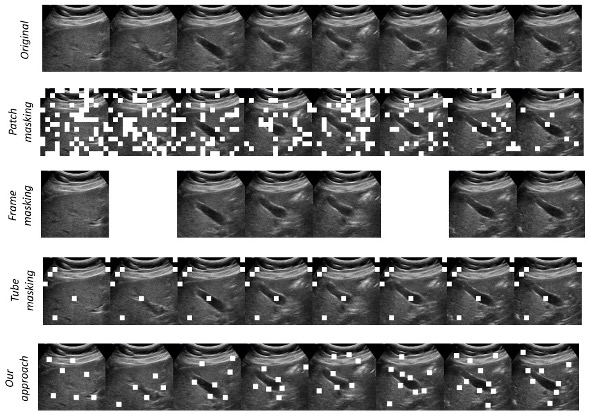
\includegraphics[width=\linewidth]{figs/focusmae/teaser_patch.jpg}
        \caption{}
        \label{focusmae_fig:teaser_a}
    \end{subfigure}
    %
	\begin{subfigure}[b]{0.45\linewidth}
		\centering
		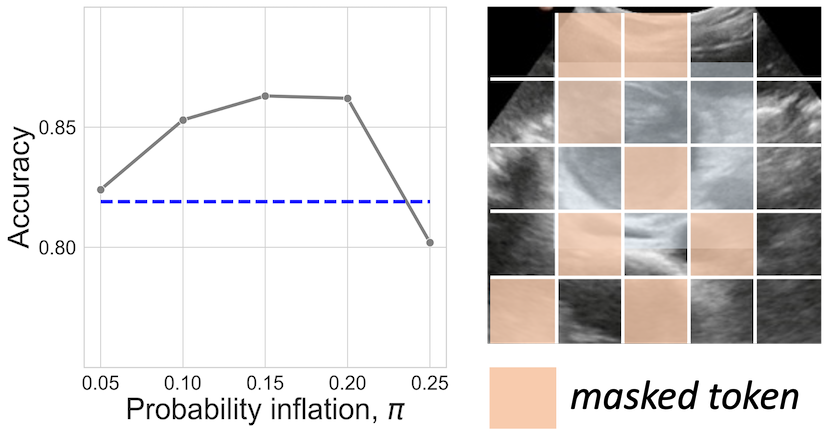
\includegraphics[width=0.95\linewidth]{figs/focusmae/obj_prior.png}
		\caption{}
		\label{focusmae_fig:teaser_b}
	\end{subfigure}
    \caption[Masking strategy of FocusMAE and its motivation]{(a) Masking strategy of FocusMAE in comparison to existing random patch \cite{maest}, frame \cite{wei2022masked}, tube \cite{videomae} masking. Our masking approach selects more tokens from the semantically meaningful regions with a small number of background tokens for masking. (b) Effect of increasing masking probability on object regions. We inflate the masking probability of the tokens which spatially lie within the object region (gray region) by $\pi$. However, excessive masking of the object region degrades performance. The blue line shows the accuracy of the original random masking. }
    \label{focusmae_fig:teaser}
\end{figure}

\mypara{Our Proposal}
%
In USG videos, the spatiotemporal regions indicative of malignancy typically constitute a humble portion. Notice that these are high information regions as opposed to non-GB portions of the frames, which are low information regions. 
Thus, random masking (uniform distribution) is not conducive to learning effective representations of malignancy. The random selection of masked tokens introduces redundant background information, necessitating a more systematic approach. Few recent approaches suggest using an adaptive mask sampling strategy for more meaningful semantic representation \cite{adamae, mgmae}. MGMAE \cite{mgmae} suggests using object motions to guide the mask sampling. AdaMAE \cite{adamae} exploits a policy gradient optimization strategy by the maximization of the expected token reconstruction error in order to boost the sampling probability of the tokens belonging to the objects. Since the organs are mostly stationary in USG videos or CT volumes, the motion-guided strategy is not applicable to our case. On the other hand, our experiments show that AdaMAE does not perform significantly better than VideoMAE. By focusing solely on reconstruction error, the model may underrepresent crucial features or patterns within the data. In contrast, we adopt a simple strategy called \focusmae to effectively mask the high-information patches in the input to learn better disease representation. We identify semantically meaningful candidate high-information regions, and systematically bias the sampling strategy with these region-priors to sample the masking tokens from these focused candidate regions. By using a stronger masking on the high information regions, and reconstructing these tokens, \focusmae learns a more refined representation of GBC. %malignancy. 

\par We validate the \focusmae method on a curated dataset which contains the 64 videos from the GBUSV dataset (refer to \cref{data:gbusv}), and 27 additional malignant videos. Since our idea of focused masking is generic, we validate the generality of the method by applying it to a public CT-based Covid identification task \cite{covidctmd}.

\mypara{Contributions} 
%
The key contributions of this chapter are:
%\vspace{-0.5em}
\begin{enumerate}[label=\textbf{(\arabic*)}]
%\itemsep-0.6em
	\item We posit that existing SOTA techniques for GBC detection in USG images exhibit suboptimal accuracy and generalization performance. Image-centric methodologies demonstrate shortcomings in capturing the intricate representations inherent in video data. Singular images may lack the requisite features for unambiguous malignancy categorization. Consequently, we advocate for a paradigm shift toward video-based GBC detection for USG. 
	%Image-centric methodologies demonstrate shortcomings in capturing the intricate representations inherent in video data. Singular images may lack the requisite features for unambiguous malignancy categorization. Further, image-based techniques exhibit efficacy primarily in small-scale datasets. Our experiments reveal that they fail to generalize effectively to larger, unseen data. In response, we employ masked autoencoder-based representation learning to discern malignant features from USG video sequences for GBC detection.
	%
	\item Even though video-based GBC classification shows improvement over image-based methods in terms of accuracy, specificity, and sensitivity, we observe that the random masking in MAE presents opportunities for further improvement. Notably, the spatiotemporal regions indicative of malignancy typically constitute a small portion of the video. The random selection of masked tokens introduces redundant background information, necessitating a more systematic approach. To address the issue, we propose a novel design, \focusmae, to systematically bias the masking token selection from the semantically meaningful candidate regions. As a result, the network is compelled to learn a more refined representation of GB malignancy while reconstructing the masked tokens. %We report an accuracy of 96.4\% using our approach as against 84\% by the current SOTA of GBCNet \cite{basu2022surpassing} and Radformer \cite{basu2023radformer}\footnote{Both GBCNet and RadFormer gave an identical accuracy in our experiments. We confirmed that individual predictions were not identical.}
	%
	\item Our idea of focused masking is generic, and we validate the generality of the method by applying it to a public CT-based Covid identification task \cite{covidctmd}. %We report an accuracy gain of 2.9\% by our method over the SOTA \cite{videomaev2}.
    %
	%\item Concurrently, we curate the most extensive USG video dataset available for GBC detection. We establish the dataset by adding 27 USG video samples exhibiting GBC to the publicly available GBUSV dataset. The dataset will be made available to the community. 
    %
    %\item We also note that the problem of USG video-centric detection of GBC with machine learning was not previously attempted in literature. We provide the first solution to the problem and present a strong baseline. 
\end{enumerate}


\section{Related Work}
%
\myfirstpara{Deep Learning for GB related Diseases}
%
Several studies have leveraged DNNs to detect various GB conditions, including calculi, cholecystitis, and polyps, using diagnostic images. For instance, \cite{gbYolo} applied YOLOv3 to identify the GB and stones in CT images. \cite{gbPolyp} focused on GB segmentation and employed an AdaBoost classifier for polyp diagnosis. Meanwhile, \cite{gbPolyp2} concentrated on classifying neoplastic polyps in cropped gallbladder ultrasound (USG) images, utilizing an InceptionV3 model. Additionally, \cite{jang2021diagnostic} employed ResNet50 to diagnose polypoidal lesions through endoscopic USG.

\mypara{DNNs for GBC Detection}
%
Despite numerous studies on DNNs for gallbladder-related diseases, only a few have explored AI-based detection of GBC. Chang \etal \cite{chang2022ct} employed a UNet-based denoising approach to enhance the image quality of Low-Dose CT scans for characterizing GBC, focusing primarily on segmentation methods. In contrast, Basu \etal \cite{basu2022surpassing} introduced a specialized CNN architecture called MS-SoP and a Gaussian blurring-based curriculum for efficient GBC detection in USG images. Gupta \etal \cite{gbc-lancet} further uses the MS-SoP architecture for a patient subgroup study on a large prospective patient cohort. \cite{basu2023radformer} exploits a transformer-based dual-branch architecture with bag-of-word style feature embedding for accurate and explainable GBC detection. \cite{basu2022unsupervised}, on the other hand, utilizes unsupervised contrastive learning to learn malignancy representations. 
%
Despite the above studies, we observe a notable gap in the literature regarding models for video-based GBC detection from USG videos. This gap in research motivates the current work.

%\mypara{Deep Learning for USG Modality}
%
%DNN models have found extensive applications in USG imaging tasks, including the detection of ovarian cancer \cite{zhang2019improved}, identification of breast cancer regions, masses, and boundaries \cite{cao2019BreastLesion,ning2020multi, zhu2020second}, as well as the measurement of head circumference in fetal ultrasound images \cite{sobhaninia2019FetalHC, budd2019FetalHC}. 

\mypara{Video-based Classification and Recognition}
%
Transformers have seen an influx over CNNs in recent years due to their superior performance. Transformers with combined spatiotemporal attention \cite{vivit}, hierarchical spatiotemporal attention \cite{videoswin}, and separable spatial and temporal attention \cite{timesformer, vidtr} are popular for video-based recognition or classification. %Additionally, related areas of study in weakly-supervised video classification encompass video action recognition \cite{TSN}, temporal action localization \cite{actionformer}, and anomaly detection \cite{weaklypolyp}. 

\mypara{Masked Autoencoder for Videos}
MAEs have gained popularity for self-supervised video representation learning (SSL). \cite{maest, videomae} extend the MAE from image to video domain. \cite{omnimae} used a combined image and video-based MAE pipeline. On the other hand, \cite{qing2023mar} introduced running cell masking to reduce cost. Another study \cite{videomaev2} recommended masking decoder tokens as well. \cite{adamae} recommends an adaptive masking strategy instead of random masking. Some studies look for priors like motion trajectory \cite{mgmae,patrick2021keeping, Sun_2023_CVPR}. \cite{li2022semmae} recommends using semantic parts guided MAE. \cite{maskvit} introduces the usage of both spatial and spatiotemporal attention along with variable token masking ratio.


\begin{figure*}[t]
    \centering
    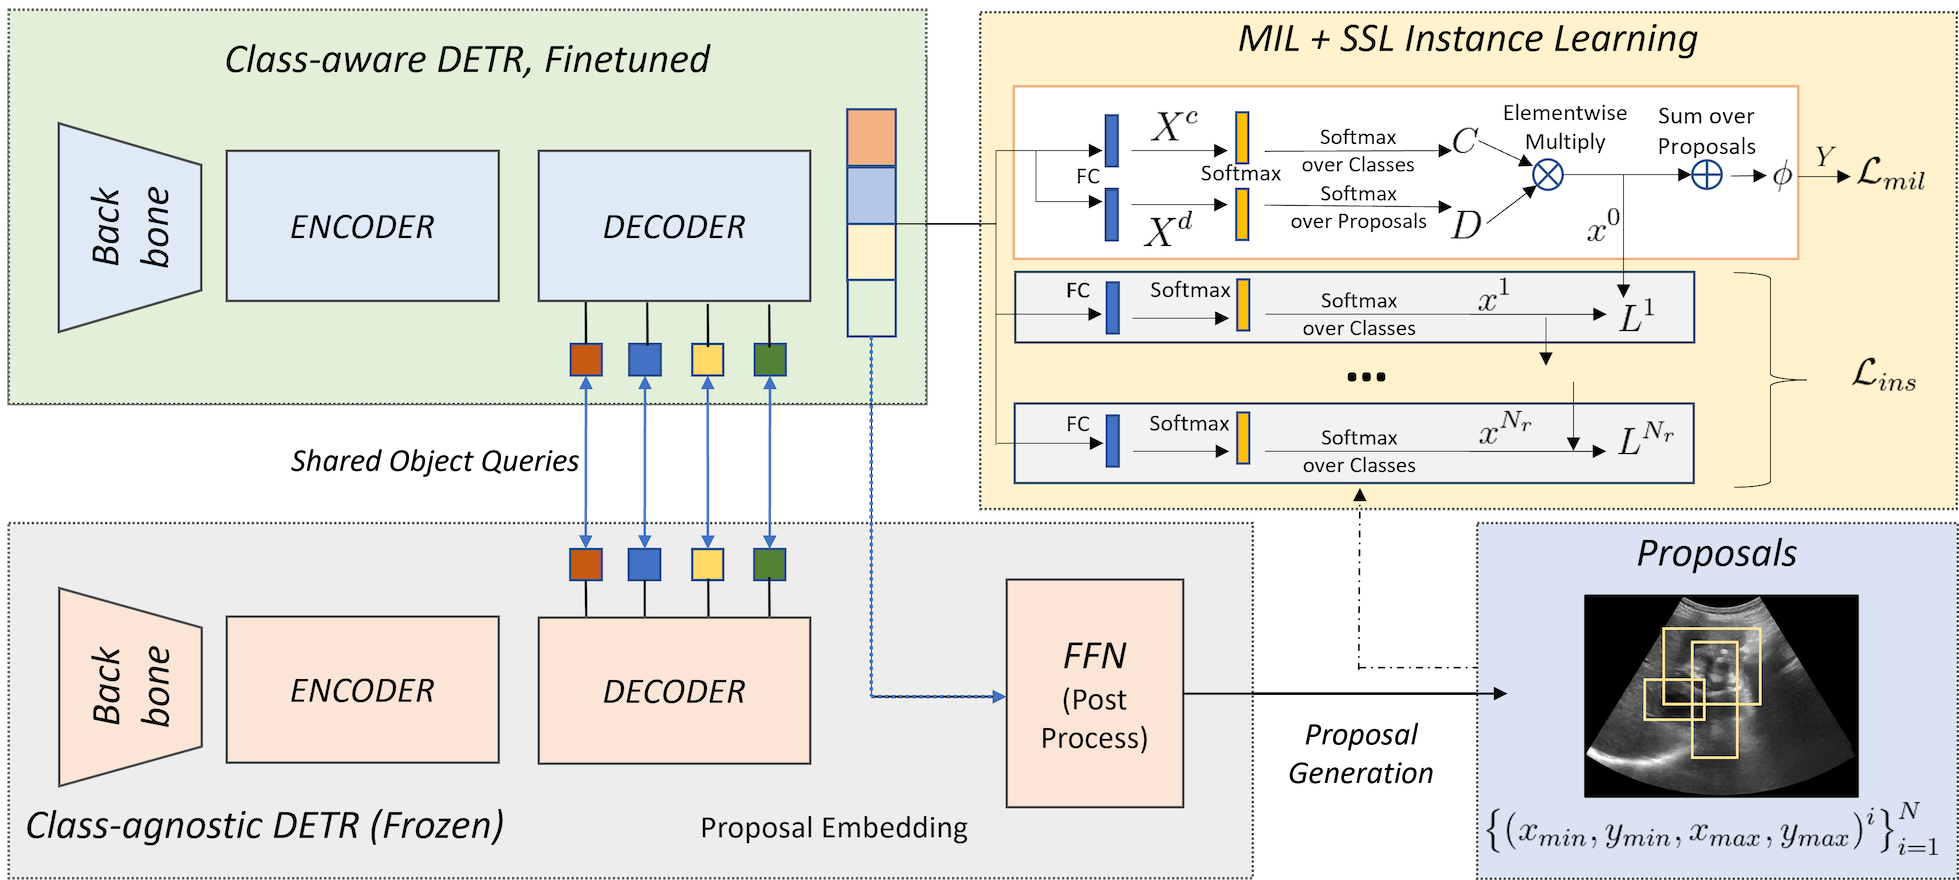
\includegraphics[width=\textwidth]{figs/arch.png}
    \caption{Overview of the proposed FocusMAE pipeline. Our design proposes guiding the masking tokens with the localization of the candidate focus regions containing high-information. The systematic biasing with focused high-information region priors helps to build a more meaningful reconstruction task for disease representation learning. }
    \label{fig:enter-label}
\end{figure*}

\section{Proposed Method}
\begin{figure*}[t]
    \centering
    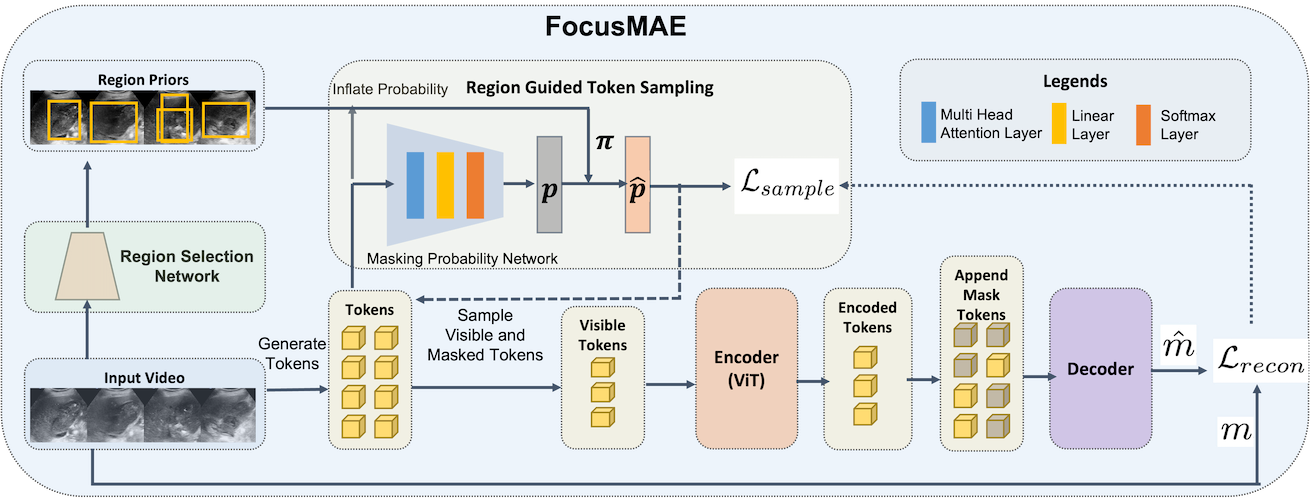
\includegraphics[width=\textwidth]{figs/focusmae/arch.png}
    \caption[Overview of the FocusMAE pipeline]{Overview of the FocusMAE pipeline. Our design proposes guiding the masking tokens with the localization of the candidate focus regions containing high-information. The systematic biasing with focused high-information region priors helps to build a more meaningful reconstruction task for disease representation learning. }
    \label{focusmae_fig:arch}
\end{figure*}

\subsection{Object Priors in MAE}
%
Visual data often demonstrate sparser semantically meaningful information distribution dominated by the foreground objects. Current MAE techniques predominantly use random masking, which may result in sub-optimal performance as the information may not be uniformly distributed. For the USG videos, GBC often occupies a very small portion of the frames. Random masking mostly biases the networks to learn representations of redundant backgrounds containing other organs or abdominal cavities. To alleviate the issue, %we advocate exploiting the object location priors with high information density to enhance the representation learning in MAE. 
we advocate leveraging the object localization priors characterized by high information density to enhance the representation learning in MAE.
We show in \cref{focusmae_fig:teaser_b} the preliminary evidence of potential advantages of boosting the masking token probability with object localization priors. We selected a random validation split containing about 20\% of our GB USG Video dataset. We used the malignant ROI boxes provided in the dataset to specify object locations. We manually increased the masking probability of patches within the bounding box region for the data samples, and used them for self-supervised pretraining. We varied the probability boosting values, denoted by $\pi$, representing the increased probability for patches within the bounding box region as compared to the patches from the background. Our experiment reveals that elevating the probability of masking for patches from the bounding box region, as opposed to random masking, leads to a noticeable enhancement in results. %However, highly inflating the masking probability for patches from the bounding box region may compromise the integrity of the pretext task and result in performance degradation. 
However, excessively inflating the masking probability for patches from the bounding box region may compromise the integrity of the pretext task and consequently lead to performance degradation.
These findings underscore the importance of recognizing that distinct image patches contribute differently to the learning of visual representations. Furthermore, the emphasis on reconstructing foreground objects with a balanced approach is crucial for optimal performance.

\subsection{\focusmae Architecture}
%
\label{sec:method_subsample}
\mypara{Video Sub-sampling}
% 
Video data contains temporal redundancy as the consecutive frames see a very high overlap in content. We sub-sample the videos to reduce the temporal redundancy. Assuming a video containing $F$ frames, we first sub-sample $\frac{F}{4}$ frames with a stride of $4$. Although the viewpoint in USG frames can change very quickly, in our observation of the data, the changes within the frames at a distance equivalent to a stride of 4 from each other are insignificant. Each frame has a size of $3\times H\times W$, $H$, and $W$ stands for the height and width of the frame having three channels (RGB). We further divide these sub-sampled frames for a video into clips -- each clip containing 16 frames. We then randomly sample four clips to use during the pretraining phase. Before passing to the pretraining pipeline, the frames are resized to $224\times 224$.

\mypara{Token Generation}
% 
We first divide a video $V$ of size $T\times 3\times H\times W$ into non-overlapping cubic tokens of size $2\times 3 \times 16 \times 16$. $T$ is the number of frames (temporal dimension), $H$ and $W$ are the height and width of the frames. Each frame has RGB channels. We use a 3D convolution of kernel size = $(2, 3, 16, 16)$,  stride $(2, 16, 16)$, and $d$ output channels. Using this 3d convolution layer, we generate a total of $N=\frac{T}{2}\times\frac{H}{16}\times\frac{W}{16}$ tokens, each of dimension $d$ ($d=384$ in our design) for every video. 
%Next, we add the positional information to the tokens using the fixed 3D periodic positional encoding scheme introduced in \cite{vaswani2017attention}.
Subsequently, we incorporate positional information into the tokens utilizing the fixed 3D periodic positional encoding as introduced in \cite{vaswani2017attention}.

\mypara{Generating Object Localization Priors}
%
We employ deep object detection networks as the region proposal network (RPN) to detect the potential gallbladder region within a frame. The predicted bounding boxes are used as potential candidate regions containing the objects (malignancy). We used the public GBCU \cite{basu2022surpassing} dataset for training the object detectors. The GBCU dataset provides USG images with regions-of-interest marked with bounding boxes. The training focuses on two classes: background and the GB region. We lower the confidence threshold of the predicted boxes to generate multiple candidate regions. These regions are used as priors in a masking token sampler to boost the masking probability of the tokens. If a token's spatial central point falls within the region prior, then its masking probability is inflated. To define a candidate region for an entire clip, we take the union of the candidate regions for each frame within the clip.

\mypara{Masked Token Sampling with Region Priors}
%
To generate the masking probabilities for the tokens, we follow \cite{adamae} and use an auxiliary network consisting of Multi-Head Attention (MHA) with a Linear and a Softmax ($\sigma$) layer following it. Given the embedded tokens $x \in \mathbb{R}^{N \times d}$, the probability scores $p \in \mathbb{R}^N$ over all tokens is generated as follows:
\begin{align}
z = \text{MHA}(x); \quad z \in \mathbb{R}^{N \times d} \\
p = \sigma(\text{Linear}(z)); \quad p \in \mathbb{R}^N
\end{align}
Region priors then boost the probability score as follows:
\begin{align}
\hat{p}_i = p_i + \pi_i 
\end{align}
If the $i$-th token spatially lies within the candidate regions, then we inflate the masking probability of the token by $\pi_i \in(0,\delta)$, where $\delta$ is a small fraction less than $0.25$. 
Subsequently, we choose a set of visible token indices $\mathcal{V} \in {1,\ldots,N}$ without replacement, with a probability of $(1-\hat{p}_i)$ for the $i$-th token. The set of masked token indices, denoted by $\mathcal{M}$, is derived from the complement set of $\mathcal{V}$ within the range ${1,\ldots,N}$, and is given by $\mathcal{M} = \{1,\ldots,N\} \setminus \mathcal{V}$. The number of sampled visible tokens, denoted as $N_v$, is calculated as $N(1 - \rho)$, where $\rho \in (0, 1)$ is a predefined masking ratio. 
%We then select without replacement a set of visible token indices $\mathcal{V} \in \{1,\ldots,N\}$ with the probability $(1-\hat{p}_i)$ for the $i$-th token. The set of masked token indices is given by $\mathcal{M} = \{1,\ldots,N\} \setminus \mathcal{V}$. The number of sampled visible tokens $N_v$ is computed based on a pre-defined masking ratio $\rho \in (0, 1)$ and equals $(1 - \rho)N$.

\mypara{Encoder}
%
For computational efficiency, only the visible tokens are passed to the encoder. The number of visible tokens is $N_v = (1-\rho)N$. We employed a vanilla ViT architecture with space-time attention \cite{timesformer}. The ViT encoder has a depth of 12 layers with 6 heads in each layer. The embedding dimension is 384. 

\mypara{Decoder}
%
The encoded visible tokens are appended with the masked token before passing to the decoder. We keep the decoder depth to 10 after grid searching for optimal depth. The masked tokens are learnable. Usually, the decoder in an MAE architecture is a shallow and narrow ViT. However, our experiments indicate that increasing the decoder depth can help in performance gain. The decoder takes the encoded tokens with the learnable masked tokens and reconstructs the original video cube of size $\frac{T}{2}\times\frac{H}{16}\times\frac{W}{16}$.

\subsection{Training}
%
We use two different loss functions in the \focusmae pre-training phase. The masking reconstruction loss is the primary objective for the MAE-based pre-training framework. On the other hand, we employ a token sampling loss to generate the token sampling probability. At the fine-tuning stage, a cross-entropy loss is used (refer to \cref{sec:focusmae_impl}).

\mypara{Masking Reconstruction Loss} 
%
We have employed the \emph{Mean Squared Error} loss (MSE), measuring the disparity between the predicted and ground-truth RGB values of the masked tokens, as the objective function for pretraining the MAE. The loss function is given as:
\begin{align}
   \mathcal{L}_{recon} = \frac{1}{|\mathcal{M}|}\sum_{i \in \mathcal{M}}||\hat{m}_i - m_i||_2 
\end{align}
Here $\hat{m}$ and $m$ denote the predicted RGB values and the normalized ground-truth RGB values of the token, respectively. $|\mathcal{M}| = \rho N$ refers to the number of masked tokens. %The normalization is done at the patch level, with the mean and variance of the patch.

\mypara{Token Sampling Loss}
%
We use a token sampling loss, $\mathcal{L}_{sample}$, to train the sampling network that generates the sampling probability. We adapt the sampling loss proposed by AdaMAE \cite{adamae} and use maximization of the average reconstruction error to define the loss. The formulation of such a formulation is motivated by the expected reward maximization of the REINFORCE algorithm. %Here, the visible token sampling process is the \emph{action}, the MAE is the \emph{environment}, and the masked token reconstruction error is the \emph{return}. The reconstruction error is high in the high information regions as compared to the low information background regions. Thus, maximizing the expected reconstruction error would result in the network predicting a higher probability score for a high information region. 
In this context, the sampling process of visible tokens serves as the \emph{action}, the MAE acts as the \emph{environment}, and the error in masked token reconstruction represents the \emph{return}. Notably, the reconstruction error tends to be more pronounced in high-information regions compared to low-information background areas. Consequently, maximization of the expected reconstruction error would prompt the network to assign a higher probability score to a high-information region. The loss formulation is as follows:
\begin{align}
    \mathcal{L}_{sample} = - \sum_{i\in \mathcal{M}} \big(\log{\hat{p}_i} \cdot ||\hat{m}_i - m_i||_2 \big)
\end{align}
One key difference with the loss in AdaMAE is that the token probability in our formulation is augmented by the region priors, while AdaMAE uses a token probability for a distribution over the entire image. Thus, we obtain a more refined version of the adaptive token sampling. The log probability tackles the underflow and floating point errors. The gradient flow in the sampling network is kept independent from the ViT encoder and decoder of the main MAE. 

\begin{table}[t]
	\centering
    \footnotesize
	%\resizebox{ \linewidth}{!}{%
	\begin{tabular}{llcccc}
		\toprule
		{\textbf{Group}} & {\textbf{Method}} & {\textbf{Backbone}} & {\textbf{Acc.}} &  {\textbf{Spec.}} & {\textbf{Sens.}} \\
        %& {\textbf{Time/Frame (ms)}}\\
		\midrule
		%
        \multirow{2}{*}{Human Experts} 
		& Radiologist A  & -- & 0.786$\pm$0.134 & 1.000$\pm$0.000 & 0.672$\pm$0.201 \\%& 21.54\\
		%
		& Radiologist B  & -- & 0.874$\pm$0.088 & 1.000$\pm$0.000 & 0.811$\pm$0.126 \\%& 74.58\\
		\midrule
		\multirow{10}{*}{Image-based} 
		& ResNet50 \cite{resnet} & CNN & 0.711$\pm$0.091 & 0.822$\pm$0.102 & 0.672$\pm$0.147 \\%& 21.54\\
		%
		& InceptionV3 \cite{inception} & CNN & 0.734$\pm$0.089 & 0.953$\pm$0.072 & 0.647$\pm$0.107 \\%& 74.58\\
		%
        & Faster-RCNN \cite{fasterrcnn} & CNN & 0.757$\pm$0.058 & 0.687$\pm$0.056 & 0.808$\pm$0.091 \\%& 96.03\\
		%
		& EfficientDet \cite{efficientdet} & CNN & 0.789$\pm$0.084 & 0.761$\pm$0.099 & 0.828$\pm$0.061 \\%& 238.65\\
		%
        \cmidrule{2-6}
        & ViT \cite{vit} & Transformer & 0.796$\pm$0.068 & 0.751$\pm$0.128 & 0.820$\pm$0.076 \\%& 24.62\\
		%
		& DEIT \cite{touvron2021training} & Transformer & 0.829$\pm$0.034  & 0.787$\pm$0.154 & 0.845$\pm$0.058 \\%& 23.52\\
		%
		& PVTv2 \cite{wang2021pvtv2} & Transformer & 0.831$\pm$0.041 & 0.857$\pm$0.167 & 0.834$\pm$0.068  \\%& 32.77\\
        \cmidrule{2-6}
        & GBCNet \cite{basu2022surpassing} & CNN & 0.840$\pm$0.105 & 0.843$\pm$0.204 & 0.843$\pm$0.072 \\%& 24.62 \\
		%
		& US-UCL \cite{basu2022unsupervised} & CNN & 0.808$\pm$0.127 & 0.871$\pm$0.217 & 0.776$\pm$0.109 \\%& 21.54 \\
        %& Weakly_DETR \cite{basu2022unsupervised} & CNN & 0.808$\pm$0.127 & 0.871$\pm$0.217 & 0.776$\pm$0.109 \\
		%
		& RadFormer (SOTA) \cite{basu2023radformer} & Transformer & 0.840$\pm$0.105 & 0.776$\pm$0.162 & 0.877$\pm$0.088 \\%& 32.77 \\
		%
		\midrule
		\multirow{5}{*}{Video-based} 
        %& ViViT \cite{vivit} & Transformer & $\pm$ & $\pm$ & $\pm$ & \\
		%
        & Video-Swin \cite{videoswin} & Transformer & 0.925$\pm$0.053 & \textbf{1.000$\pm$0.000} & 0.903$\pm$0.085 \\%&  \\
		%
        & TimeSformer \cite{timesformer} & Transformer & 0.920$\pm$0.058 & 0.967$\pm$0.067 & 0.909$\pm$0.058 \\%&  \\
        %
        & VidTr \cite{vidtr} & Transformer & 0.924$\pm$0.038 & \textbf{1.000$\pm$0.000} & 0.800$\pm$0.072 \\%& \\
		%
		& VideoMAEv2 \cite{videomaev2} & Transformer & 0.942$\pm$0.066 & 0.937$\pm$0.078 & 0.940$\pm$0.120 \\%&  \\
		%
		& AdaMAE \cite{adamae} & Transformer & 0.947$\pm$0.053 & 0.952$\pm$0.066 & 0.913$\pm$0.116 \\%& \\
		%
		\cmidrule{2-6}%[1.5pt]
		& \focusmae (Ours) & Transformer & \textbf{0.964$\pm$0.072} & 0.940$\pm$0.120 & \textbf{1.000$\pm$0.000} \\%& \\
		\bottomrule
	\end{tabular}
	%}
	\caption[Comparison of SOTA and \focusmae for GBC detection]{The 5-fold cross-validation (Mean$\pm$SD) accuracy, specificity, and sensitivity of baselines and \focusmae in detecting GBC from the USG. \focusmae achieves the best accuracy and perfect sensitivity, which is much desired for GBC detection. We also report how the expert radiologists perform in detecting GBC from the video dataset. The radiologists were blinded from accessing any patient-related data or clinical/ histopathological findings. The radiologists classified each video using the Gallbladder Reporting and Data Standard (GB-RADS) \cite{gb-rads-paper}. Our model outperforms human radiologists in detecting GBC from USG videos. Recall that our ground truth labels are biopsy-proven. The performance of the expert radiologists in our study is comparable to literature \cite{gbc-lancet}. 
    %We have also added the average time per frame during inference in milli-seconds (when run in a 32GB V100 GPU) to compare the speed of detection.
    }
	\label{tab:main}
\end{table}


\section{Dataset }
%
\subsection{Curated USG Video Dataset for GBC Detection}
%
\begin{figure}[t]
    \centering
    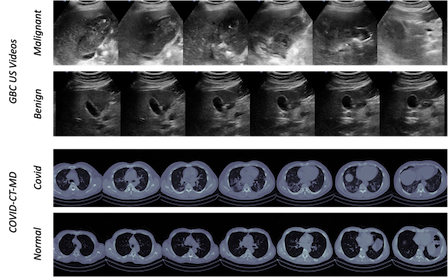
\includegraphics[width=0.85\linewidth]{figs/focusmae/data_sample_med.png}
    \caption[Sample video sequences from the USG and CT datasets]{Sample video sequences from our USG video dataset used for GBC detection, and the public COVID-CT-MD dataset \cite{covidctmd}. We show samples of both malignant and benign (non-malignant) sequences for GBC data. For the covid data, we show sample sequences for both Covid and non-Covid categories.}
    \label{focusmae_fig:data_sample}
\end{figure}
\mypara{Video Data Collection and Curation}
%
We utilized both the public Gallbladder USG video dataset (GBUSV) \cite{basu2022unsupervised} and an additional set of USG videos collected by our team of radiologists. The GBUSV dataset comprises 64 Gallbladder USG videos, with 32 labeled as benign and another 32 labeled as malignant. To augment our dataset for the video-based \gbc detection task, we incorporated 27 additional USG videos specifically depicting Gallbladder malignancy. We relied on the GB biopsy reports for labeling the videos. We cropped the video frames from the center to safeguard patient privacy and annotations. The processed frames have a size of 360x480 pixels. The data collection process is discussed in detail ealier in \Cref{data:gbusv}. \cref{focusmae_fig:data_sample} shows sample sequences from the dataset. 

%We obtained video samples from patients referred to a tertiary care referral hospital for abdominal USG examinations targeting suspected Gallbladder pathologies. Each patient provided informed written consent during recruitment, and we ensure patient privacy by fully anonymizing the data. The institute Ethics Committee approved the study. Patients were fasting for a minimum of 6 hours to ensure adequate distention of the \gb. Our team of radiologists employed a 1-5 MHz curved array transducer (C-1-5D, Logiq S8, GE Healthcare) for the scanning process. The scanning protocol covers the entire gallbladder (including fundus, body, and neck) and any associated lesions or pathologies. 

%\mypara{Annotation}
%
%The video labels in GBUSV are already provided. For our additional videos, we relied on the GB biopsy reports for labeling. Additionally, two radiologists with 2 and 10 years of expertise in abdominal ultrasound (USG), were consulted to draw bounding boxes covering the entire GB and the adjacent liver parenchyma in the video frames.  
%The radiologists were pinpoint frames exhibiting clinical signs of malignancy. 
%In cases of malignant videos, the radiologists reached a consensus to label each frame as either malignant or non-malignant. 
%Although these frame-level annotations aren't directly employed for training video-based detection methods, they play a crucial role in qualitatively assessing the detectors. Moreover, these annotations hold potential for frame-level Video Anomaly Detection tasks. 
%Additionally, in each video, the radiologists have drawn an axis-aligned bounding box covering the entire GB and adjacent liver parenchyma to annotate the Region-of-Interest (ROI) that may contain the malignancy.


\mypara{Dataset Statistics}
%
The dataset comprises 59 malignant and 32 non-malignant videos, collected from 41 malignant and 32 benign patients, respectively. In total, the dataset encompasses 21,955 frames, with 18,406 frames attributed to videos labeled as malignant. %Among these, radiologists identified 3212 frames exhibiting definite signs of malignancy. 

\mypara{Dataset Splits}
%
We report the 5-fold cross-validation metrics for the complete dataset for key experiments. The cross-validation splits were conducted on a patient-wise basis, ensuring that all videos of a patient appeared exclusively in either the training or the validation split.

\subsection{Public CT Dataset for Covid Detection}
%
We use the publicly available COVID-CT-MD dataset \cite{covidctmd} to assess the generality of our proposed method. The COVID-CT-MD dataset contains lung CT scans of 169 (108 male and 61 female) confirmed positive COVID-19 cases, 76 (40 male and 36 female) normal cases and 60 (35 male and 25 female) Community-Acquired Pneumonia cases. All samples are annotated at the patient, lobe, and slice levels by three different radiologists. The authors used a Siemens SOMATOM Scope scanner to obtain the scans with the output size of the reconstructed images set to $512\times512$ pixels. 
Additionally, the dataset also contains clinical data, including the patient's age, gender, weight, symptoms, surgery history, follow-up and RT-PCR test reports. However, during our experiments, we did not use the clinical data. 
We used a stratified random 80:20 split to get the training and validation data.

\section{Implementation and Evaluation}
\label{sec:focusmae_impl}
In this section we discuss the specific training setup with FocusMAE for our GBC detection task. We use the FocusMAE-based pretraining on the ViT encoder, enabling it to learn disease representation for the downstream GBC classification task. Following this pretraining phase, the ViT network is fine-tuned for the GBC classification task using classification loss. The pretraining and fine-tuning details including the hyperparameters are discussed here.

\mypara{Pretraining}
%
We implemented our experiments using PyTorch \cite{paszke2019pytorch}. We used Kinetics-400 pretrained weights for MAE weight initialization. Although there is a domain gap in natural and medical image data, studies show that pretraining on natural image data improves network performance on medical imaging tasks \cite{alzubaidi2020transferlearning, cheng2017transfer}.
We used the video sub-sampling scheme discussed in \cref{sec:method_subsample}. We apply random-resize cropping, random horizontal flipping, and random scaling as part of the data augmentations for pretraining. We chose ViT-S as the backbone. 
We use $2 \times 3 \times 16 \times 16$ sized patches on the input video which has size $16\times3\times224\times224$. Consequently, we obtain $\frac{16}{2} \times \frac{3}{3}\times \frac{224}{16} \times \frac{224}{16} = 1568$ tokens for each video.
%We use patch size of $2 \times 3 \times 16 \times 16$, resulting in $\frac{16}{2} \times \frac{3}{3}\times \frac{224}{16} \times \frac{224}{16} = 1568$ tokens for an input video of size $16\times3\times224\times224$.  
The pretraining phase is trained with an AdamW optimizer with LR $0.0001$, layer decay $0.75$, and weight decay $0.05$, for minimizing the MSE loss over 300 epochs. The batch size was 2. Warm-up was done for 3 epochs with LR $0.001$.

\mypara{Fine-tuning}
%
\label{label:impl_ft}
For sub-sampling the videos during fine-tuning, a denser sample rate of 3 was used. We used 16 frames to constitute a clip. From each video, we sampled 5 clips uniformly. During inference, we predict the labels for each of the clips. If any of the clips is predicted as malignant, the entire video is labelled as malignant. We minimized a soft-target cross entropy loss using an AdamW optimizer with LR $10^{-5}$, layer decay $0.75$, and weight decay $0.05$ for 30 epochs. We used a batch size of 4. 

We have used a machine with an Intel Xeon Gold 5218@2.30GHz dual-core processor and 8 Nvidia Tesla V100 32GB GPUs for our experiments. 

\mypara{Evaluation Metrics}
%
We used video-level accuracy, specificity (true negative rate), and sensitivity (true positive rate/ recall) for assessing the video-based GBC identification. %We have used 5-fold cross-validation. 


\begin{figure}[t]
    \centering
    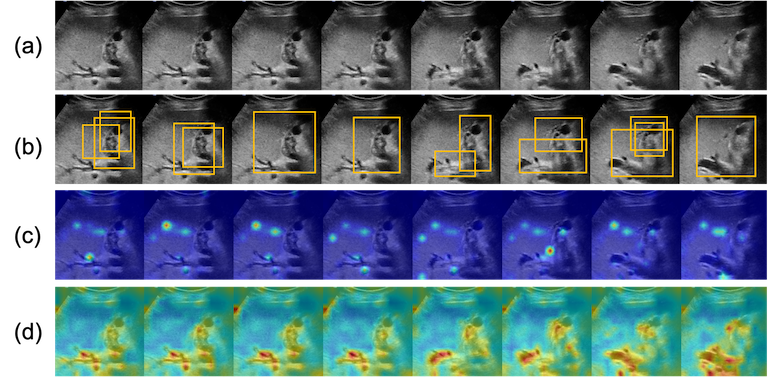
\includegraphics[width=\linewidth]{figs/vis_gbc_focusmae.png}
    \caption[Visual demonstration of the benefit of using the \focusmae]{Visual demonstration of the benefit of using the \focusmae method for GBC detection. (a) Original frames from a USG video sequence exhibiting GB malignancy. (b) Candidate regions as prior (in yellow). (d), (e) Attention visualization for the downstream malignancy detection for VideoMAE and \focusmae, respectively. For \focusmae, the attention is well guided to the key regions containing the malignancy, as opposed to VideoMAE.}
    \label{focusmae_fig:qualitative}
\end{figure}

\begin{figure}[!ht]
    \centering
    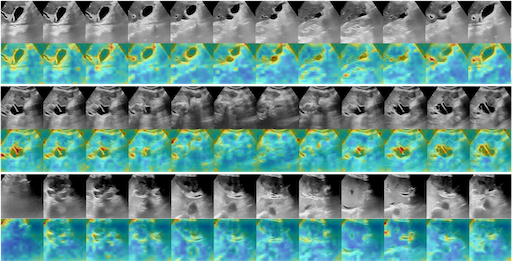
\includegraphics[width=\linewidth]{figs/vis_attention_gbc.png}
    \caption[Attention visuals for \focusmae for GBC detection]{Attention visuals for \focusmae for the GBC detection task on the USG videos. We show three different maligant video samples. For each video sample, the upper row shows the sequence with the original frames, and the lower row shows the attention on the frames.}
    \label{focusmae_fig:visual_supp_gbc}
\end{figure}

\section{Experiments and Results}
%
\subsection{Efficacy of \focusmae over SOTA Baselines}
%
We explore the GBC classification performance on USG videos for five SOTA video classification methods, namely Video-Swin \cite{videoswin}, TimeSformer \cite{timesformer}, VidTr \cite{vidtr}, VideoMAEv2 \cite{videomaev2}, and AdaMAE \cite{adamae}. 

In addition, we have also explored our previously developed SOTA techniques \cite{basu2022surpassing, basu2023radformer, basu2022unsupervised} that are specialized for GBC detection on USG images. Apart from these specialized models, we analyze the performances of popular image-centric CNN-based classifiers \cite{resnet,inception} and detectors \cite{fasterrcnn, efficientdet}. We also look into three popular Transformer-based classifiers - ViT \cite{vit}, DEiT \cite{touvron2021training}, and PvT \cite{wang2021pvtv2} for GBC detection. 


\mypara{Using Image-based Methods for Video Classification}
%
We use the same video sub-sampling scheme used during the fine-tuning phase (ref. \cref{label:impl_ft}) of the \focusmae to get the frames and clips. We then use the image-centric methods to predict the labels for each frame in the clips. If the majority of the frames in a clip are predicted as malignant, then the clip is predicted as malignant. If any clip within a video is predicted as malignant, the overall video is categorized as malignant. The image-based methods were pretrained on the public GBCU \cite{basu2022surpassing} dataset. 

\mypara{Quantitative Analysis}
%
We show the 5-fold cross-validation performance in terms of accuracy, specificity, and sensitivity for the baselines and the proposed \focusmae in \cref{tab:main}. Clearly, the video-based techniques trump the image-centric SOTA methods of GBC detection, supporting our recommendation of a paradigm shift to video-based classification for the problem. Additionally, we see the effectiveness of the \focusmae in detecting GBC. 


\mypara{Qualitative Analysis}
%
We show the qualitative analysis in \cref{focusmae_fig:qualitative}. The random masking by VideoMAE does not adequately mask the high-information malignant region. In contrast, the region prior guided \focusmae generates stronger masking for learning the malignant representation by biasing the masking towards the malignancy localization region. We visualize the attention rollout during the downstream task. Clearly, \focusmae's attention regions highlight semantically more meaningful areas, such as the gallbladder boundary and anatomical structures, compared to VideoMAE. More visuals for FocusMAE attention is shown in \cref{focusmae_fig:visual_supp_gbc}.

\subsection{Generality of the Proposed Method}
%
\begin{table}[!t]
    \footnotesize
	\centering
	%\resizebox{ \linewidth}{!}{%
	\begin{tabular}{llccc}
		\toprule
		{\textbf{Group}} & {\textbf{Method}} & {\textbf{Acc.}} &  {\textbf{Spec.}} & {\textbf{Sens.}} \\
		\midrule
		%
		\multirow{5}{*}{Image-based} 
		& ResNet50 \cite{resnet} & 0.721 & 0.739 & 0.711 \\
		%
		& InceptionV3 \cite{inception} & 0.672 & 0.739 & 0.632 \\
        %
        %& USG-UCL \cite{basu2022unsupervised} & 0.802 & 0.869 & 0.763\\
		%
        \cmidrule{2-5}
        & ViT \cite{vit} & 0.770 & 0.783 & 0.763 \\
		%
		& DEIT \cite{touvron2021training} & 0.770 & 0.696 & 0.816 \\
		%
		\midrule
		\multirow{3}{*}{Video-based} 
        %& ViViT \cite{vivit} & Transformer & & & \\
		%
        %& Video-Swin \cite{videoswin} & 0.820 & 0.695 & 0.894 \\
		%
        & TimeSformer \cite{timesformer} & 0.787 & 0.739 & 0.816 \\
        %
        %& VidTr \cite{vidtr} & 0.443 & 0.826 & 0.210 \\
		%
		& VideoMAE \cite{videomae} & 0.852 & 0.956 & 0.789 \\
		%
		%& AdaMAE \cite{adamae} & & & \\
		%
		\cmidrule{2-5}
		& FocusMAE (Ours) & 0.885 & 0.895 & 0.869 \\
		\bottomrule
	\end{tabular}
	%}
	\caption[Comparison of SOTA and \focusmae for Covid detection]{The performance comparison in terms of accuracy, specificity, and sensitivity of baselines and \focusmae for detecting COVID from CT \cite{covidctmd}. CT-slices are analogous to the video frames, and thus, video-based detection methods are applicable to CT modality as well. Our proposed method consistently outperforms the SOTA baselines on the COVID detection task, establishing the generality and applicability of our method across two different medical imaging modalities - USG and CT. }
	\label{tab:covid}
\end{table}



\begin{figure}[!t]
    \centering
    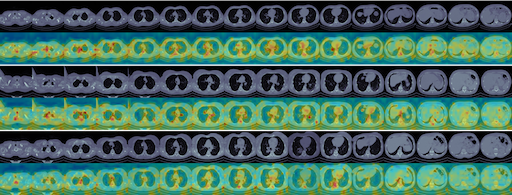
\includegraphics[width=\linewidth]{figs/vis_attn_covid.png}
    \caption[Attention visuals for \focusmae for Covid detection]{Attention visuals for \focusmae for COVID detection from CT images. We show four COVID CT samples. For each  sample, the upper row shows the sequence with the original CT slices, and the lower row shows the attention on these slices.}
    \label{focusmae_fig:visual_supp_covid}
\end{figure}

%
We explored the generality of the proposed \focusmae method on the task of Covid detection from a publicly available CT dataset \cite{covidctmd}. \cref{tab:covid} shows that \focusmae achieves much better accuracy, specificity, and sensitivity, indicating the superiority of the disease representation learning capability of \focusmae. \cref{focusmae_fig:visual_supp_covid} shows the attention visuals for COVID detection. The applicability of \focusmae on two distinct tasks -- 1) GBC detection from USG videos, and 2) Covid detection from CT -- provides evidence of generality of the method. 


\subsection{Ablation Study}
\begin{figure}[!t]
	\centering
	\begin{subfigure}[b]{0.23\linewidth}
        \centering
        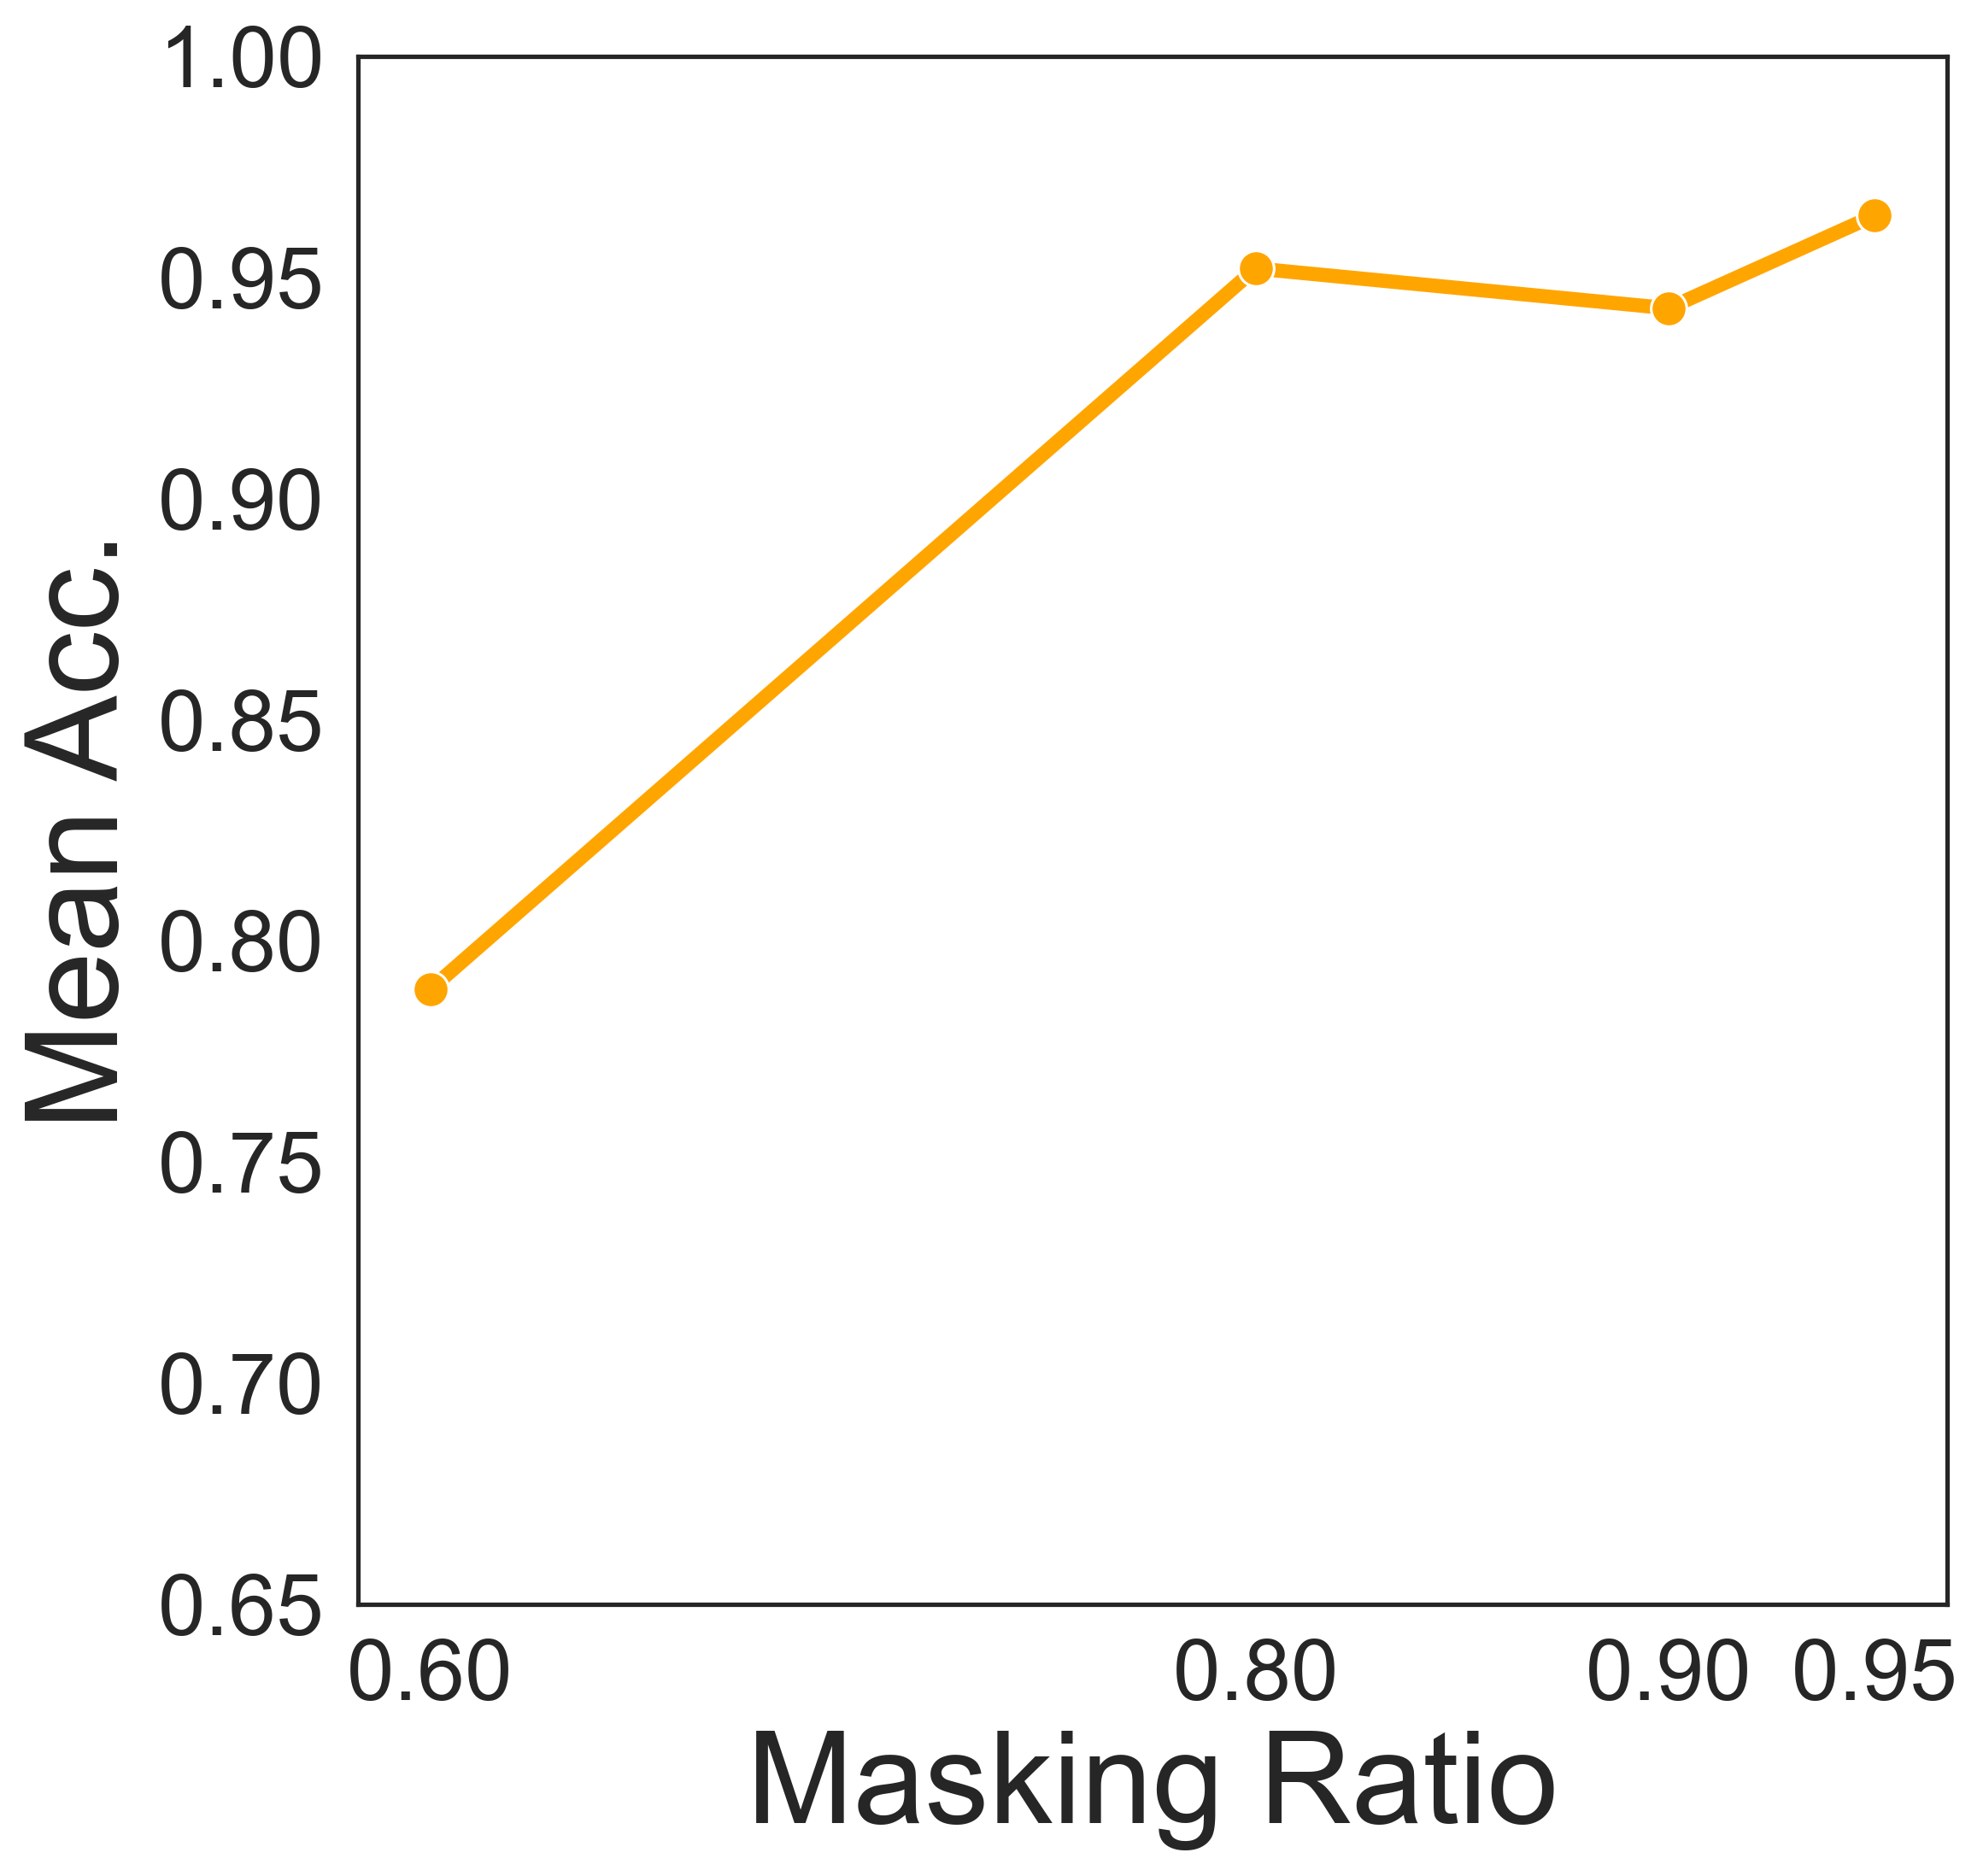
\includegraphics[width=\linewidth]{figs/focusmae/abl_mr.png}
        \caption{}
        \label{focusmae_fig:ablation_mr}
    \end{subfigure}
	\begin{subfigure}[b]{0.23\linewidth}
		\centering
		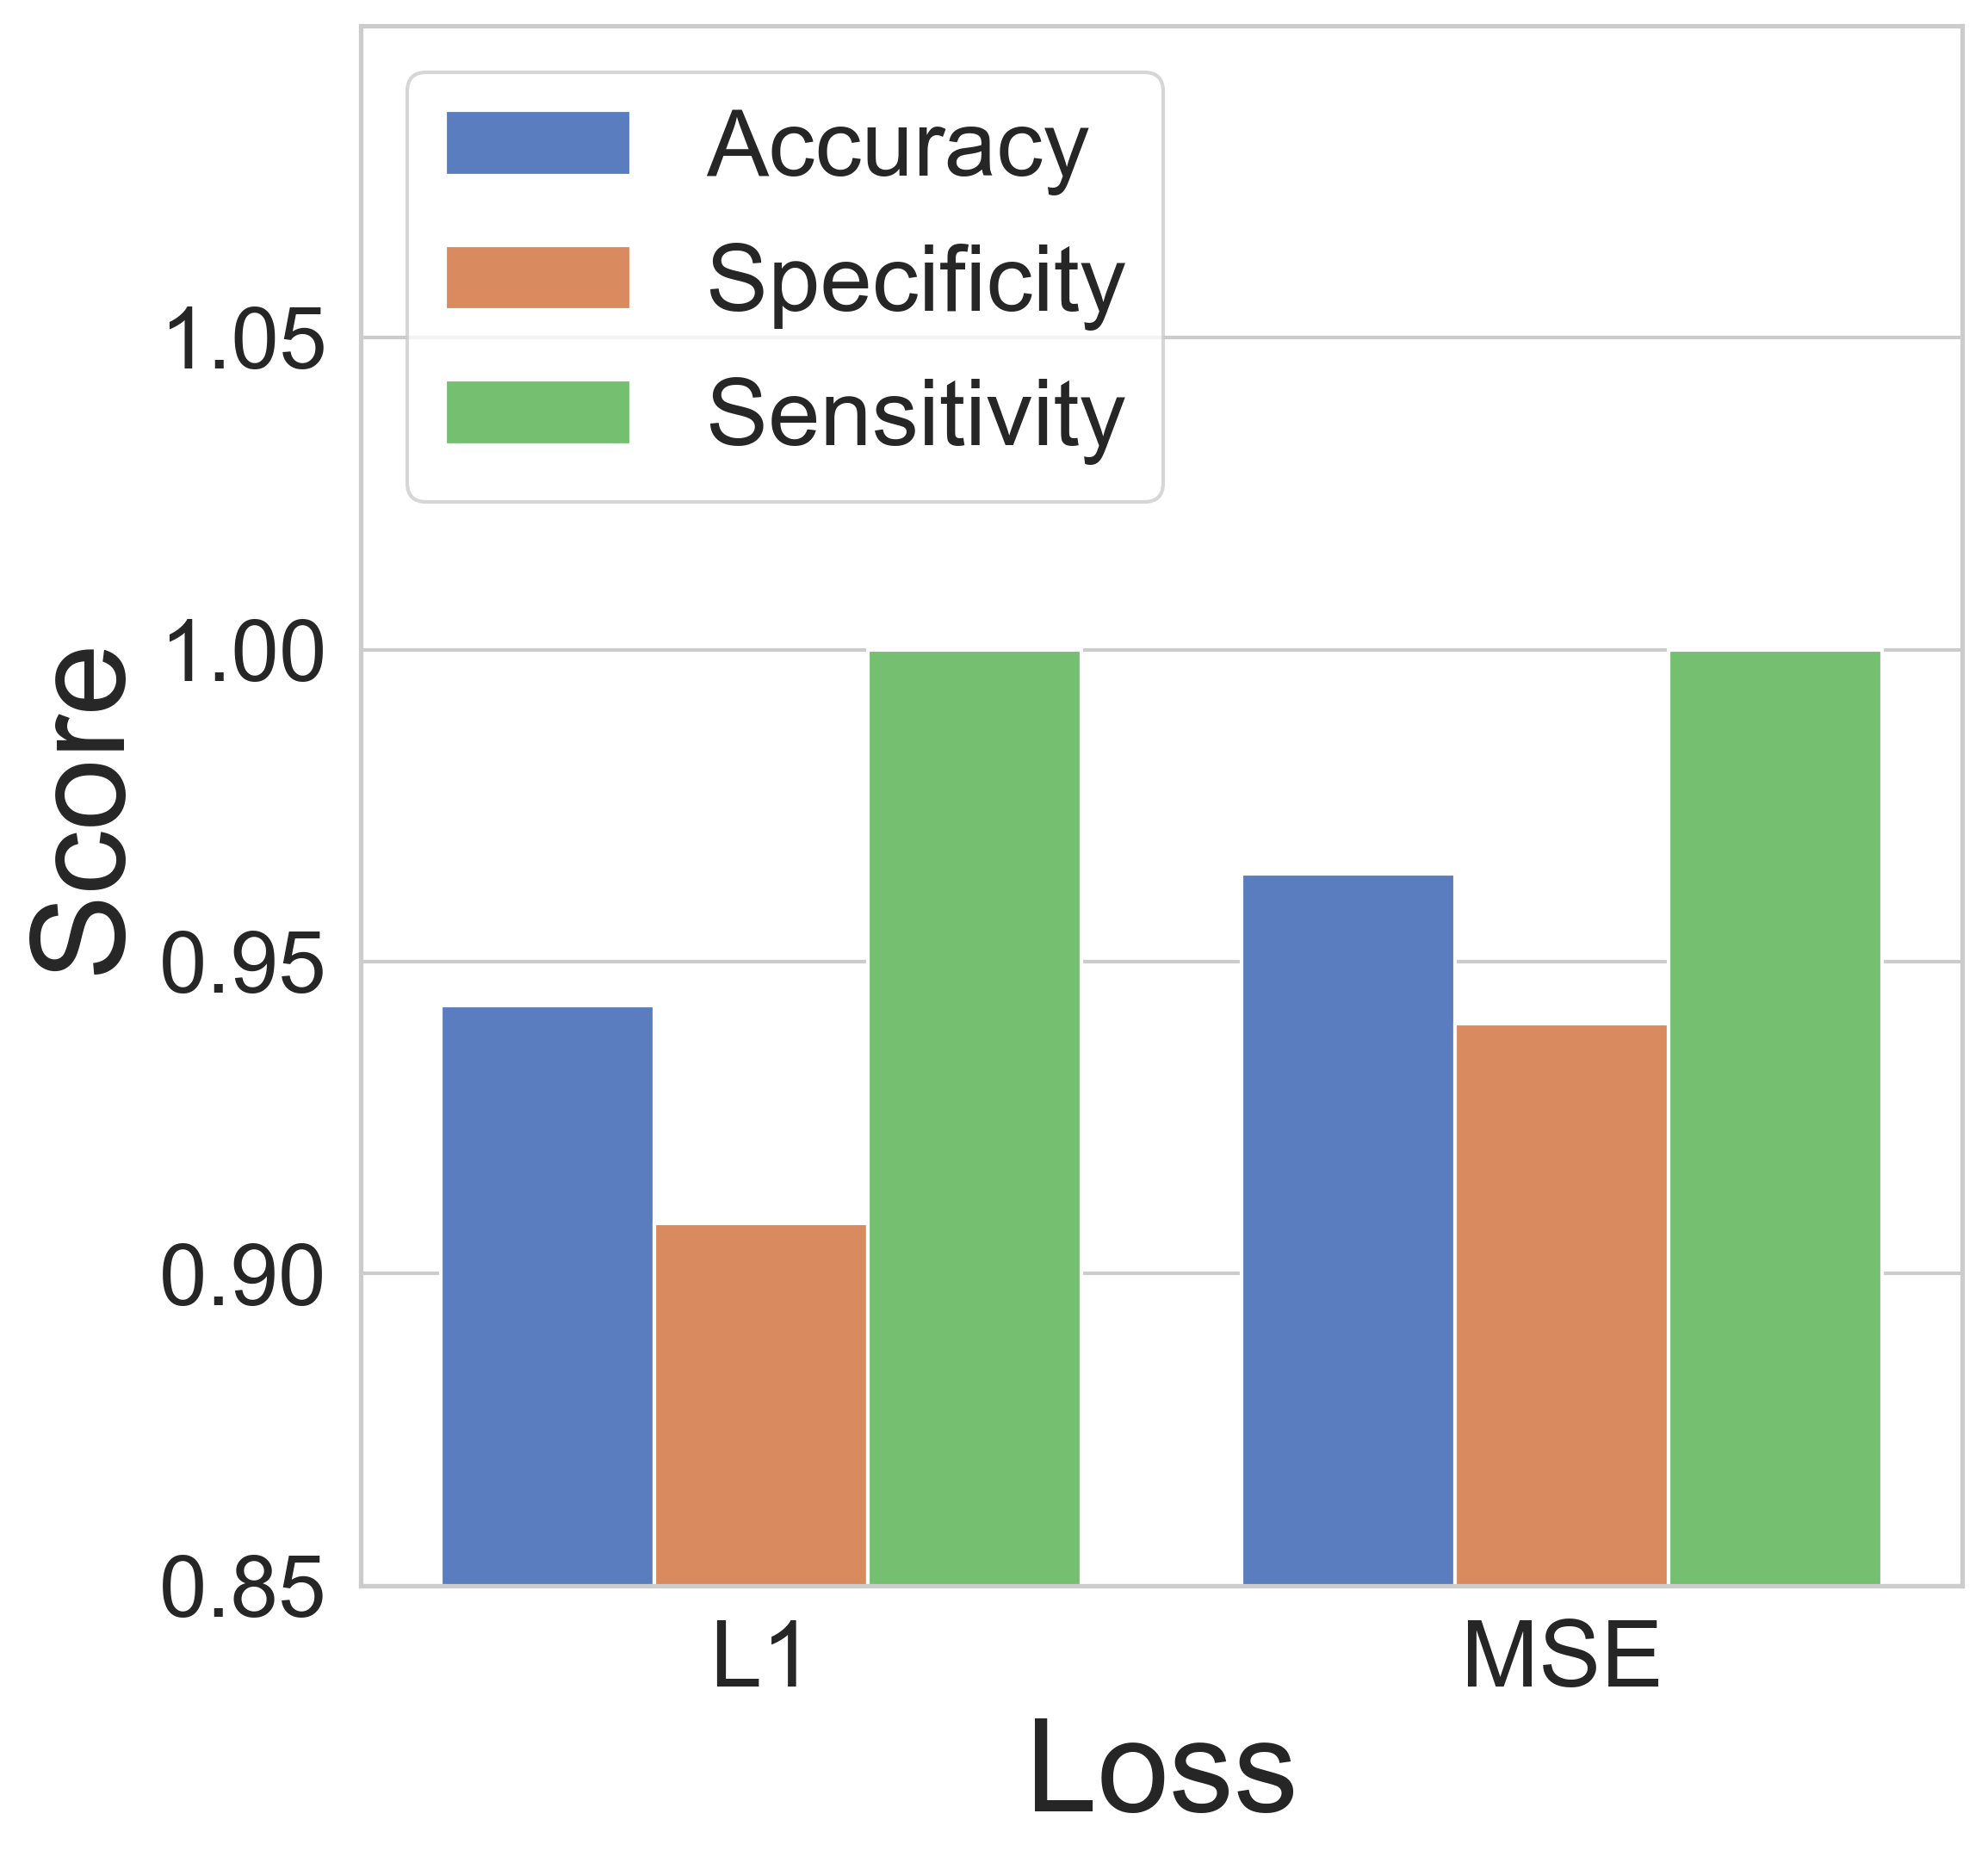
\includegraphics[width=\linewidth]{figs/focusmae/abl_loss.png}
		\caption{}
		\label{focusmae_fig:ablation_loss}
	\end{subfigure}
 %
	\begin{subfigure}[b]{0.23\linewidth}
		\centering
		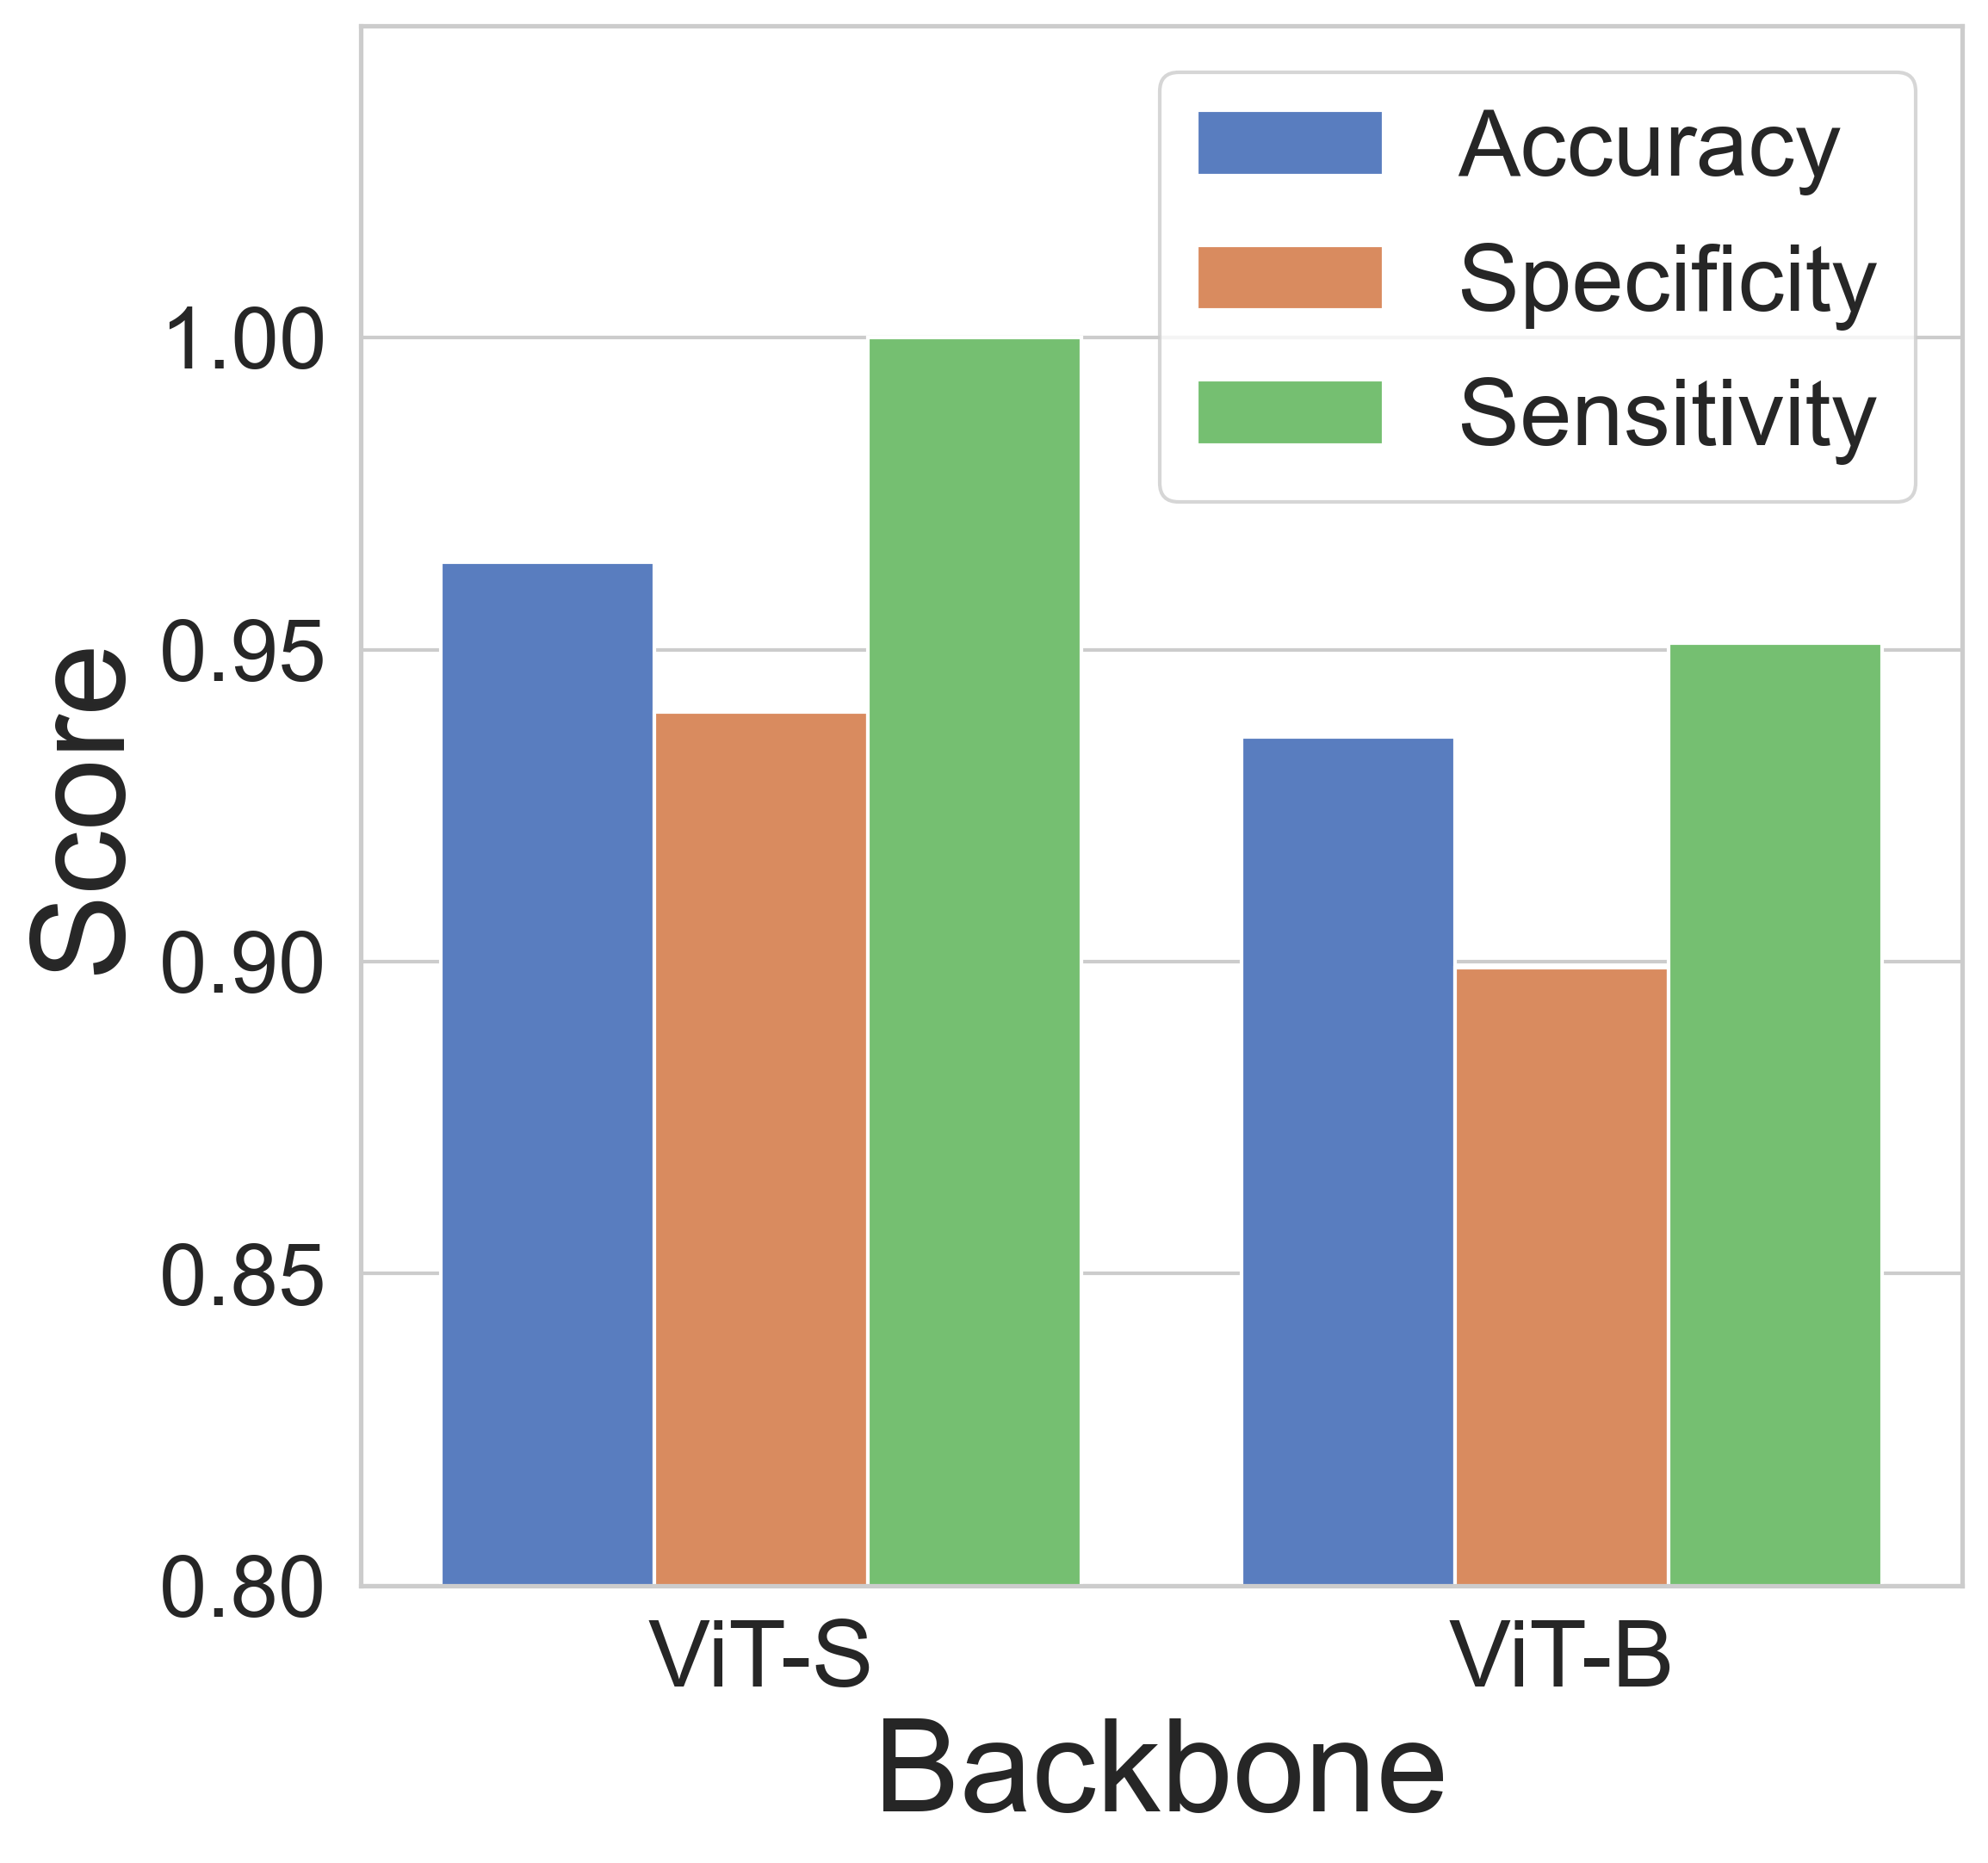
\includegraphics[width=\linewidth]{figs/focusmae/abl_enc.png}
		\caption{}
		\label{focusmae_fig:ablation_enc}
    \end{subfigure}	
    \begin{subfigure}[b]{0.23\linewidth}
		\centering
		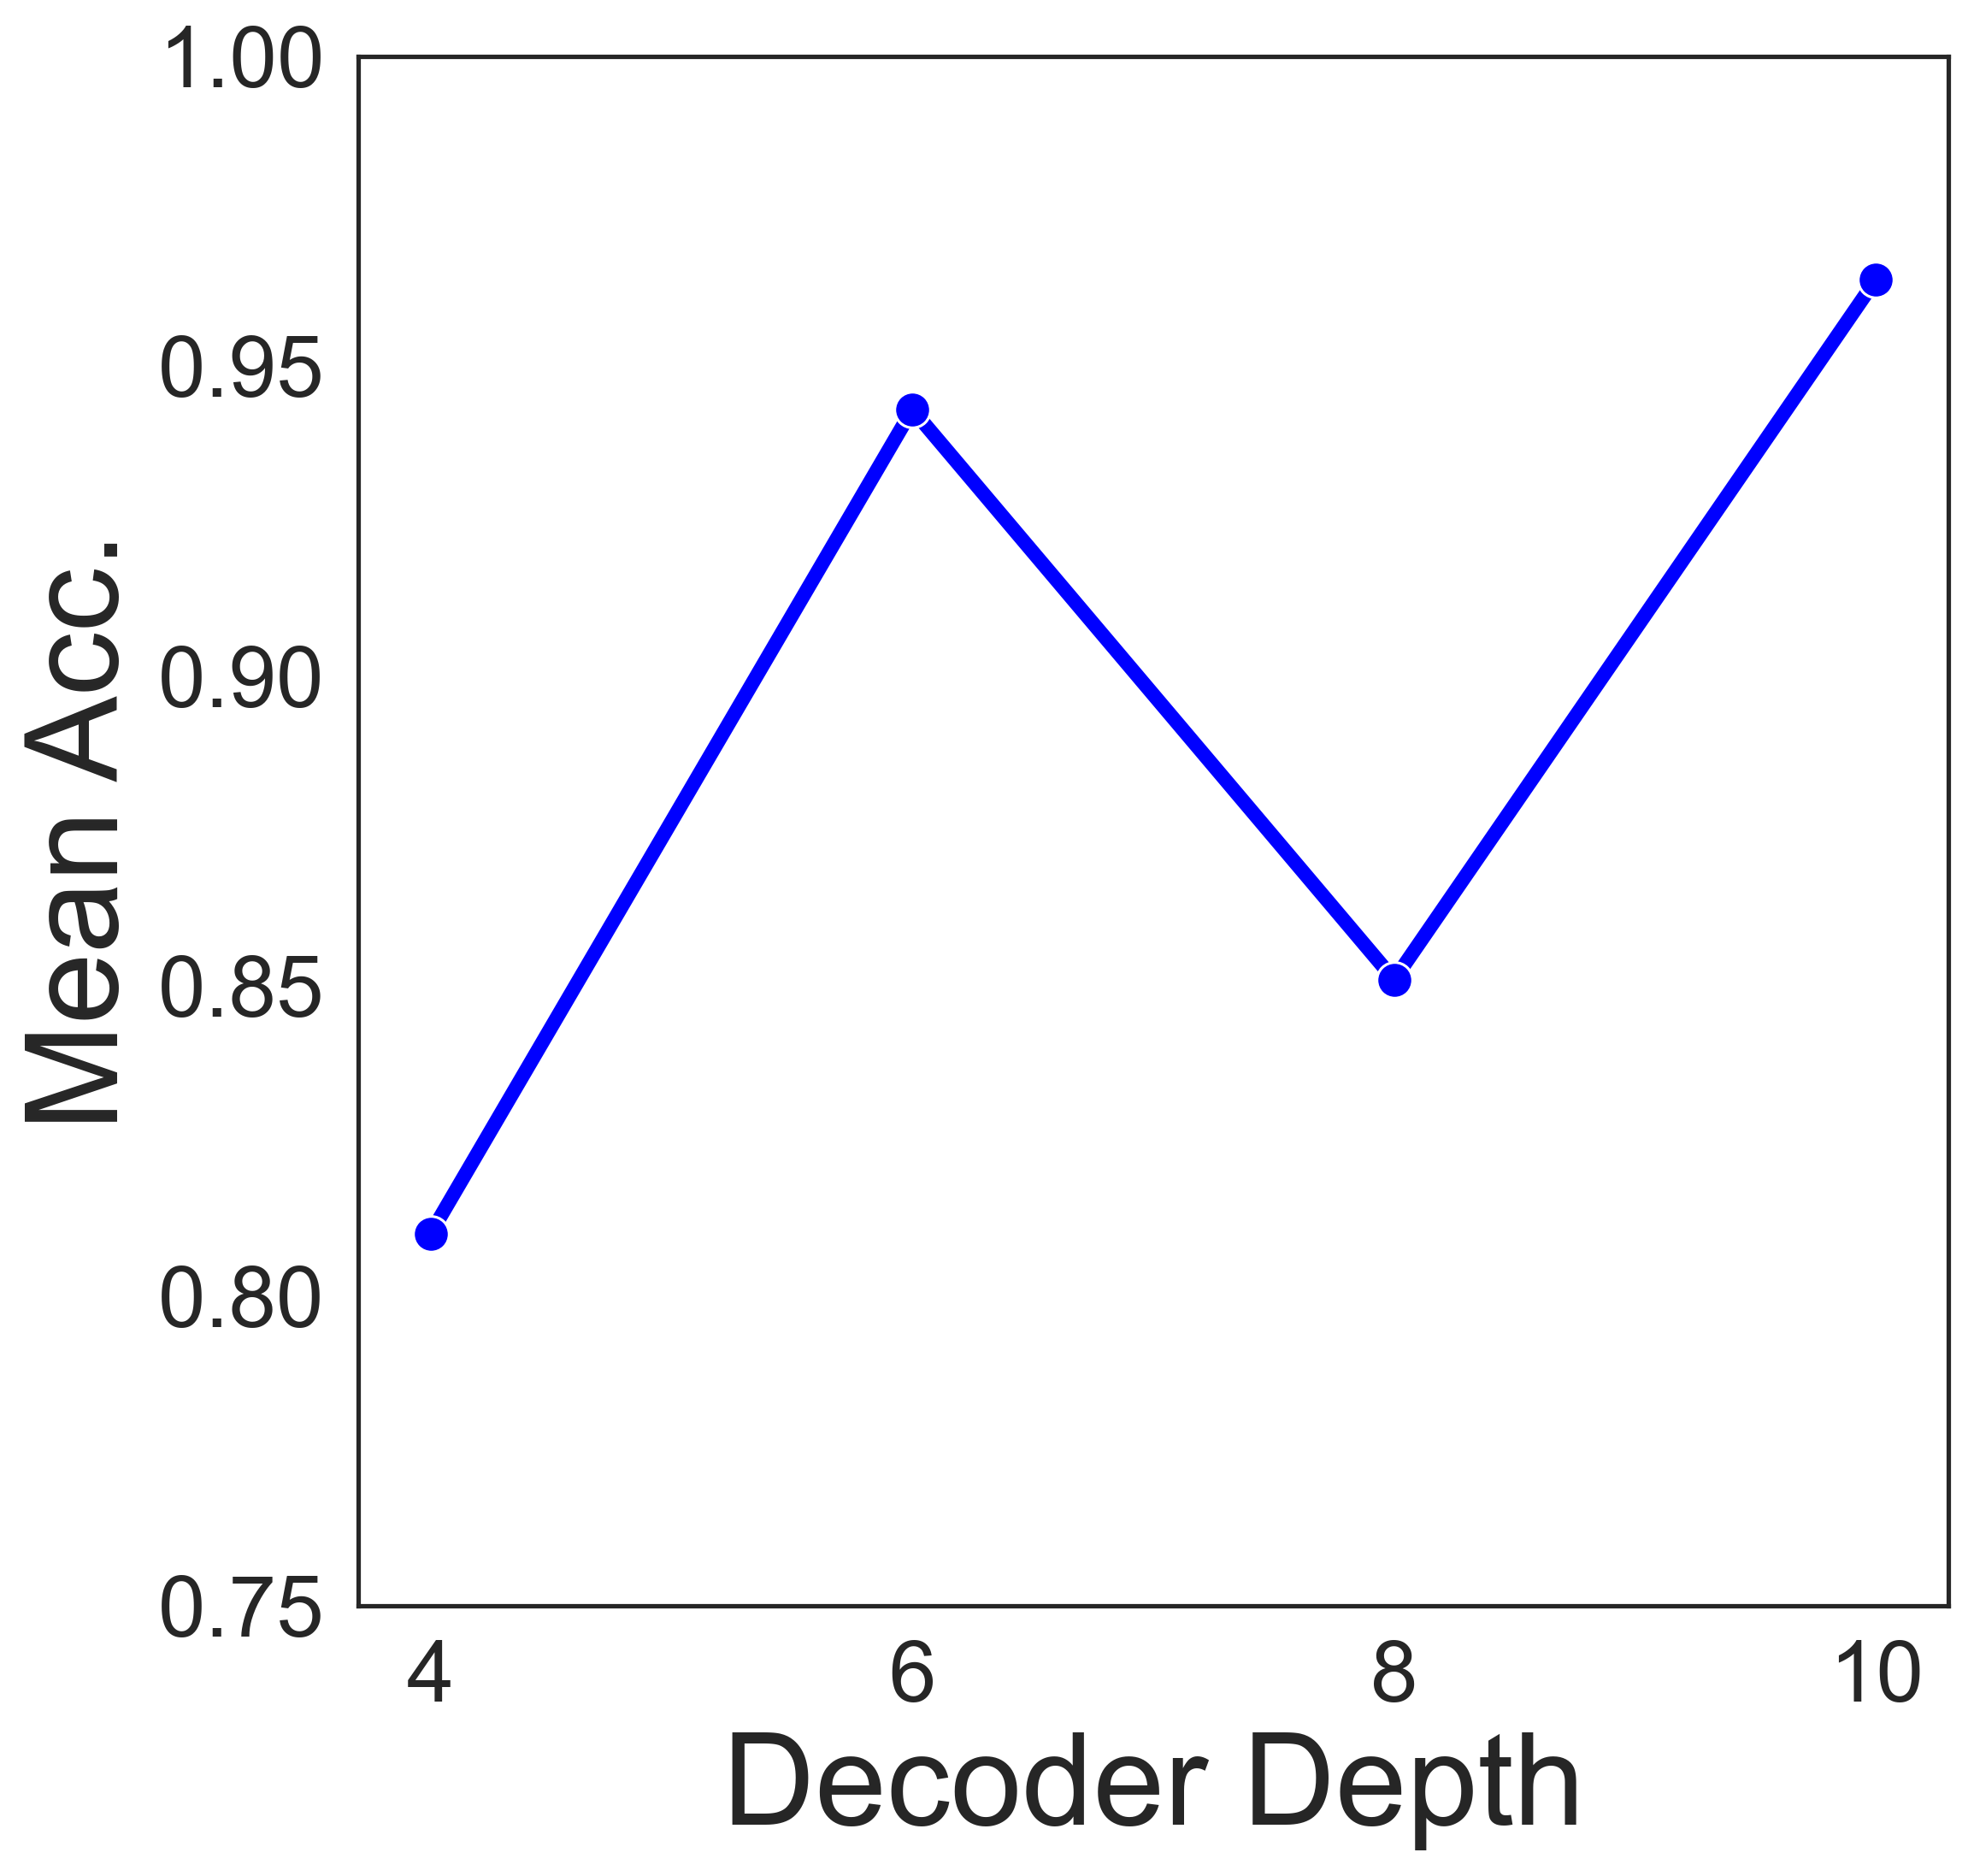
\includegraphics[width=\linewidth]{figs/focusmae/abl_dec.png}
		\caption{}
		\label{focusmae_fig:ablation_dec}
	\end{subfigure}
	\caption[Ablation study on \focusmae]{Ablation study. We report the mean scores over 5-fold cross-validation for GBC detection. (a) Effect of varying the masking ratio ($\rho$) on accuracy. (b) Effect of varying the reconstruction loss - L1 vs. MSE - for SSL pretraining. Training with MSE yields 2.2\% better accuracy. (c) Performance for different backbones. (d) Effect of varying the decoder depth on the accuracy. }
	\label{focusmae_fig:ablation}
\end{figure}

\begin{table}[!t]
	\centering
    \footnotesize
	\resizebox{ \linewidth}{!}{%
	\begin{tabular}{cccccccc}
		\toprule
		\multirow{3}{*}{\textbf{Masking Ratio}} & \multirow{3}{*}{\textbf{Decoder Depth}} & \multicolumn{6}{c}{\textbf{Loss}} \\
        & & \multicolumn{3}{c}{\textbf{MSE}} & \multicolumn{3}{c}{\textbf{L1}} \\
        & & Acc. & Spec. & Sens. & Acc. & Spec. & Sens. \\
        %& {\textbf{Time/Frame (ms)}}\\
		\midrule
		%
        \multirow{4}{*}{0.6}
		& 4  & 0.538$\pm$0.443 & 0.808$\pm $0.123& 0.940$\pm$0.120 & 0.943$\pm$0.065 
         & 0.940$\pm$0.120 & 0.938$\pm$0.076 \\
  
        & 6 & 0.952$\pm$0.071 & 0.940$\pm$0.120 & 1.000$\pm$0.000 & 0.943$\pm$0.065& 0.940$\pm$0.120& 0.938$\pm$0.076  \\
        
        & 8 & 0.942$\pm$0.066 & 0.940$\pm$0.120 & 0.938$\pm$0.076& 0.943$\pm$0.065 & 0.940$\pm$0.120 & 0.938$\pm$0.076  \\
        
        & 10 & 0.749$\pm$0.144 & 0.940$\pm$0.120 & 0.600$\pm$0.490  & 0.943$\pm$0.065 & 0.940$\pm$0.120 & 0.938$\pm$0.076  \\
		%
        \midrule 
        %
		\multirow{4}{*}{0.8}
		& 4 & 0.940$\pm$0.066  & 0.940$\pm$0.120& 0.938$\pm$0.076 & 0.86$\pm$0.124 & 0.699$\pm$0.371 & 0.940$\pm$0.120 \\
        & 6 & 0.942$\pm$0.065  & 0.940$\pm$0.120 & 0.938$\pm$0.076 & 0.943$\pm$0.065 & 1.000$\pm$0.000 & 0.938$\pm$0.076 \\
        & 8 & 0.942$\pm$0.066 & 0.940$\pm$0.120 & 0.938$\pm$0.076 & 0.978$\pm$0.027 & 1.000$\pm$0.000 & 0.938$\pm$0.076\\
        & 10 & 0.952$\pm$0.070 & 0.940$\pm$0.120 & 0.967$\pm$0.067 & 0.943$\pm$0.065 & 0.940$\pm$0.120 & 0.938$\pm$0.076 \\
		%
        \midrule 
        %
        \multirow{4}{*}{0.95}
		& 4 & 0.810$\pm$0.124 &0.940$\pm$0.120& 0.538$\pm$0.443 & 0.943$\pm$0.065 &0.940$\pm$0.120 & 0.938$\pm$0.076 \\
        & 6 & 0.943$\pm$0.065 & 0.940$\pm$0.120 & 0.938$\pm$0.076& 0.943$\pm$0.065 & 0.940$\pm$0.120 & 0.938$\pm$0.076 \\
        & 8 & 0.811$\pm$0.122&0.940$\pm$0.120 & 0.538$\pm$0.443 & 0.943$\pm$0.065 & 0.940$\pm$0.120 & 0.938$\pm$0.076 \\
        & 10 & 0.964$\pm$0.072 & 0.940$\pm$0.120 & 1.000$\pm$0.000 & 0.943$\pm$0.065& 0.940$\pm$0.120 & 0.938$\pm$0.076 \\
		%
  %       \midrule 
  %       %
  %       \multirow{4}{*}{1}
		% & 4 & 0.966$\pm$0.028 & 1.000$\pm$0.000 & 0.909$\pm$0.074 & 0.965$\pm$0.071 & 0.940$\pm$0.120 & 1.000$\pm$0.000 \\
  %       & 6 & 0.943$\pm$0.065 & 0.940$\pm$0.120& 0.938$\pm$0.076 &0.943$\pm$0.065 &1.000$\pm$0.000 &0.938$\pm$0.076  \\
  %       & 8 & 0.943$\pm$0.065 & 0.940$\pm$0.120 & 0.938$\pm$0.076 & 0.943$\pm$0.065 &1.000$\pm$0.000 &0.938$\pm$0.076  \\
  %       & 10 & 0.966$\pm$0.028 & 1.000$\pm$0.000 & 0.91$\pm$0.074 & 0.943$\pm$0.065 &1.000$\pm$0.000 &0.938$\pm$0.076 \\
		\bottomrule
	\end{tabular}
	}
	\caption[Hyperparameter tuning of \focusmae]{Hyperparameter tuning. We vary the Masking ratio, Decoder depth, and the loss function for a grid search. We report the 5-fold cross-validation (Mean$\pm$SD) accuracy, specificity, and sensitivity for \focusmae in detecting GBC from the USG.}
	\label{focusmae_tab:hyperparam_supp}
\end{table}


%
We performed the ablation study on the FocusMAE with the ViT backbone on the USG Video dataset. We show the mean scores over the 5-fold cross-validation.

\mypara{Masking Ratio}
%
\cref{focusmae_fig:ablation_mr} shows how the masking ratio $\rho$ influences the performance of \focusmae. For \focusmae, 95\% masking ratio achieves the best accuracy of 96.4\%. VideoMAE uses a 90\% masking ratio with random tube-based masking. The region-prior guided approach helps \focusmae to sample more informative tokens with lower redundancy than VideoMAE.

\mypara{Reconstruction Loss}
%
We examined the effect of varying the reconstruction loss function in our study. We experimented with two variants: Mean Absolute Error or L1-loss, and Mean Squared Error (MSE). The results, shown in \cref{focusmae_fig:ablation_loss}, indicate that using MSE loss during pretraining produces better performance in terms of accuracy. Models trained with MSE loss demonstrated a 2.2\% higher mean accuracy compared to those trained with L1 loss.

\mypara{Encoder Backbone}
%
\cref{focusmae_fig:ablation_enc} demonstrates the effect of ViT variants on the token encoding task. We experimented with ViT-S and ViT-B. We observe that larger backbones do not perform well for our data, indicating potential over-fitting.

\mypara{Decoder Depth}
%
We experiment with the number of decoder blocks and present the result in \cref{focusmae_fig:ablation_dec}. We see performance gain when the decoder depth is varied from 4 to 6. However, there is a drop in performance when the decoder depth is increased to 8. The observation is consistent with \cite{videomae, adamae}. Interestingly, when we increased the depth further, we saw an increase in accuracy, which indicates that the decoder can benefit from increasing the depth and need not necessarily be a shallow network. 

\mypara{Hyper-parameter Selection}
%
We performed a rigorous grid search for selecting the hyper-parameters. \Cref{focusmae_tab:hyperparam_supp} shows the grid search result.  

\begin{figure}[t]
    \centering
    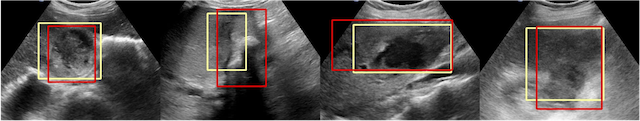
\includegraphics[width=\linewidth]{figs/focusmae/roi_vis.png}
    \caption[Visuals of candidate region priors]{Visuals of candidate regions. Red -- malignant regions identified by radiologists. Yellow -- candidate object localization generated by the RPN.}
    \label{focusmae_fig:roi}
\end{figure}

\subsection{Analysis on Candidate Region Selection}
\cref{focusmae_fig:roi} shows sample object region localization of the RPN. We adopted a FasterRCNN-based RPN for generating the candidate regions for using as priors in \focusmae. We used the GBCU dataset to pretrain the detectors for localizing the malignancy. We then lowered the threshold to generate multiple candidate regions for the video frames used in the \focusmae experiments. To calculate precision and recall in the GB localization phase, following the recommendation of \cite{ribli2018detecting}, we determine a predicted bounding box region as a true positive if its center falls within the the ground truth bounding box region. Conversely, if the center is outside the bounding box, we categorize the prediction as a false positive attributed to localization error. The RPN achieves mIoU of 0.712 with a recall rate of 0.994.

\chapter{Conclusion and Future Directions}
%
\label{chap:conclusion}
%
Finally, we come to the conclusion of the thesis. We present a concise overview of the contributions, followed by the limitations, future directions, and prospects of our work.

\par In this thesis, we have addressed the critical yet hitherto overlooked problem of Gallbladder Cancer (GBC) detection from Ultrasound Sonography (USG). We commence our exploration in \Cref{chap:intro} by discussing the background and motivation behind tackling the problem of automated detection of GBC. 
Following that, we set the stage by emphasizing USG as a diagnostic imaging modality, and its relevance in GBC diagnosis. We also highlighted the basics of USG and the unique challenges associated with USG in the context of GBC detection in \Cref{chap:usg}. \Cref{chap:data} delved into the data acquisition protocol and provided a comprehensive dataset description for the study.

\par In \Cref{chap:gbcnet}, we addressed the challenges related to \usg images, including sensor noise, acoustic shadows, echogenic textures, small pathology size, and variations in appearance of malignancy. To tackle these issues, we introduced \gbcnet \cite{basu2022surpassing}, a novel architecture specifically designed to address the complexities of \usg imaging. Employing a deep detection approach, \gbcnet initially identifies regions of interest to nullify the impact of noise. Subsequently, a novel specialized classification network (MS-SOP) is applied to learn rich representations of malignancy. Additionally, we introduced a smoothing-based curriculum inspired by the human visual acuity to train the classifier, aiming to alleviate texture bias originating from adjacent organs and tissues.

%we attack the problems associated with USG images due to the sensor noise and artifacts such as shadows and textures, and the viewpoint variations arising from the handheld sensor. We develop GBCNet \cite{basu2022surpassing}, a new architecture to solve the problems associated with USG imaging. We have used a deep detection approach to first identify the regions of interest to focus on from the image in order to nullify the effect of the noise. Following this, a novel specialized classification network (MS-SOP) is used for learning the rich representation of the cancers. In addition, we introduce a new Gaussian smoothing-based curriculum to train the classifier in order to mitigate the texture bias arising from the adjacent organs and tissues.

\par While \gbcnet exhibits significantly superior performance compared to expert radiologists and state-of-the-art CNN models, its dependence on bounding box annotations for training the detection component proves to be a bottleneck. The specialized nature of these annotations requires expert medical professionals. In response, \Cref{chap:limited} and \Cref{chap:wsod} address a crucial challenge in medical image computing -- efficient learning with limited supervised data. We explore two distinct avenues to overcome this challenge. Firstly, in \Cref{chap:limited}, we leverage unlabeled USG video data to acquire rich representations for the downstream GBC classification task on USG images \cite{basu2022unsupervised}. We introduce an unsupervised contrastive framework that exploits both intra-video and cross-video negatives, going beyond the conventional approach of mining only cross-video negatives as suggested in previous literature. Secondly, in \Cref{chap:wsod}, we formulate GBC detection as weakly supervised object detection using only image-level labels \cite{basu2023gall}. We enhance the DETR architecture with a multiple-instance learning framework, effectively addressing weakly supervised GBC detection and achieving competitive performance without the need for costly bounding box labels or additional video data.
%Although \gbcnet provides far superior performance as compared to the expert radiologists and the state-of-the-art CNN models, the reliance on the bounding box annotations to train the detection part of \gbcnet proves to be a bottleneck. The specialized nature of the annotations necessitates extensively trained medical professionals to annotate data. In response, we tackle in \Cref{chap:limited} a key challenge in the field of medical image computing -- learning efficiently with limited supervised data. We have explored two distinct avenues to solve the challenge. We exploited the unlabelled USG video data to learn rich representations for the downstream GBC classification task on USG images. We introduced an unsupervised contrastive framework to exploit both intra-video and cross-video negatives as opposed to mining only cross-video negatives as suggested in previous literature. In another approach, we formulated the GBC detection as a weakly supervised object detection using only image-level labels. We augmented the DETR architecture with the multiple instance learning framework towards solving the weakly supervised GBC detection, and achieved competitive performance even without costly bounding box labels or additional video data. 

\par In \Cref{chap:radformer}, we delve into another fundamental challenge -- interpretability. Interpretable decision-making in automated disease detection is crucial from a clinical standpoint. To meet this need, we introduce a novel deep neural network architecture, RadFormer, designed to learn interpretable representations for the detection of  GBC from USG images \cite{basu2023radformer}. RadFormer utilizes a local bag-of-word style feature embedding approach to generate explanations that are not only human-readable but also aligned with radiological reporting standards.

\par Finally, in \Cref{chap:focusmae}, we advocate a paradigm shift to USG video-based detection from the previously employed image-based detection approaches. The need to select the key individual frames in image-based detection is susceptible to operator bias, and single images may lack conclusive features of malignancy. Embracing video-based models offers clinical streamlining as they eliminate the need to select the pivotal frames and leverage rich spatiotemporal information for more accurate GBC detection.

\section{Limitations and Scope of the Work}
%
\subsection{Limitations}
\mypara{No Testing on Real-Time Patients}
%
A limitation of our study pertains to the absence of real-time patient testing, a critical aspect in ensuring the translational impact of our methodologies. The data used in the current study is retrospective in nature, and the practical applicability and robustness of our proposed solutions remain uncertain in real-time patients. Real-time patient testing introduces a dynamic environment with inherent complexities and variations that might not be fully captured in controlled experimental conditions. This limitation calls for future research efforts to bridge the gap between simulated models and actual clinical scenarios. %, promoting the development of more practical and reliable solutions for real-world healthcare applications.

\mypara{Single Center Study}
%
Our research relies on data obtained from a single medical center, and this exclusive focus introduces a limitation regarding the external validity and generalizability of our findings. It is noteworthy that our data collection center is a top tertiary care referral hospital in Northern India, attending both local and far-off patients from different states and localities. Due to this rich demographic variation, our single-center data contains a high degree of patient variation manifesting different sub-types of the disease. However, we acknowledge the limitations of single-center data in terms of limited variation in acquisition equipment and the number of radiologists involved. The dynamics within a single center may not fully encapsulate the broader variations present in diverse healthcare settings. 

\mypara{Not Identified Early Stage GBC}
%
Our work did not tackle the problem of identifying the early stage of the Gallbladder malignancy. Identifying the signs of early stage GBC to provide treatment alternatives is a desirable outcome for clinical setup. However, the aggressive nature of GBC makes the study difficult. 

\subsection{Scope of the Work and Generalizability}
In this work, we have addressed some of the key challenges such as the presence of acoustic shadows, bias to echogenic textures, small objects (pathology), variable appearance owing to non-regular anatomy, and limited data in detecting GBC from Ultrasound with DNN models. The techniques and methods developed in this thesis, such as focused regions-of-interest, smoothing-based curriculum, multi-scale features, second-order feature attention, and global-local features, address some of the key challenges inherent to ultrasound-based GBC detection. The lack of annotated data is tackled through self-supervised pretraining and weakly supervised detectors. The video-based classification method in \Cref{chap:focusmae} helps mitigate issues of operator bias.  Our techniques were demonstrated to solve the problem of GBC detection from ultrasound in the single center retrospective data settings. Nonetheless, the methods developed in this thesis address some of the core challenges of ultrasound-based GBC detection, such as presence of acoustic shadow, echogenic textures, variability in appearance owing to non-regular anatomy. We do not expect our methods to show catastrophic failure in case of unseen data. In fact, we have recently accessed image data of 9 patients (6 benign, 3 malignant) from another tertiary care hospital in Northern India, and were able to run the inference on this data using the RadFormer model (state-of-the-art image-based technique) trained on our original dataset. RadFormer showed 100\% sensitivity (all 3 malignant cases detected correctly) and 83.3\% specificity (5 out of 6 benign cases detected correctly). Although this is a minimal dataset, the results are indicative of the generalization capability of the techniques to unseen data. However, due to the acquisition shift owing to variation in ultrasound machines and operator variability, the outcomes derived from the current study may change with the diverse conditions encountered in multi-center healthcare environments, and result in performance drop. Consequently, caution should be exercised when extrapolating the results to a more extensive, varied population, emphasizing the need for future research encompassing multiple centers.% to enhance the reliability and generalizability of our conclusions.


\section{Future Directions}

\subsection{Translation to Clinical Settings}
%
In our commitment to advancing the translation of research into practical applications, we are actively engaged in exploring the real-world potential of the methodologies developed in this thesis. One avenue of implementation involves deploying the developed models and algorithms onto an Internet-of-Things (IoT) device. This initiative aims to assess the feasibility and performance of the models in a real-time, dynamic healthcare environment. We have shared the IoT device with PGIMER Chandigarh for testing on real-time patients and providing valuable insights into the adaptability and effectiveness of our proposed solutions in a clinical setting. Furthermore, to enhance accessibility and community-level impact, we have established a proof-of-concept web application. The application will be hosted on IIT Delhi's cloud infrastructure, providing a platform for radiologists within the community to leverage the developed models as a secondary resource for improved GBC detection. We seek to democratize access to advanced diagnostic tools, potentially transforming the landscape of GBC detection by empowering community-level radiologists with cutting-edge technology. %Through these practical implementations, we aim to bridge the gap between academic research and real-world healthcare applications, contributing to the development of more practical and reliable solutions.


\subsection{Domain Adaptation/ Generalization – Multi-Center Study}
%
It is imperative to address the domain shift in medical data arising from variations in patient demographics, scanning devices, and radiologist expertise across different hospitals. At present, our study is limited to a specific center, and addressing the challenge of domain adaptation or generalization is crucial for the broader applicability of our models. A future direction will be to focus on mitigating the impact of varying data distributions across hospitals, ensuring the robustness and effectiveness of our models in diverse healthcare settings. 
%To tackle the domain adaptation/generalization problem, we are actively working on the development of models capable of adapting to the nuances of hospitals across different geographic locations. This involves designing algorithms that can seamlessly generalize across diverse datasets, accounting for the inherent variations present in medical data from distinct sources.
In line with these aspirations, we have initiated efforts to acquire data from various hospitals across the country. The nationwide data collection initiative is aimed at creating a more diverse and representative dataset that encapsulates the heterogeneity present in medical data across different healthcare institutions. By incorporating data from multiple sources, we aim to enhance the generalizability and real-world effectiveness of our models, paving the way for more robust and widely applicable solutions in the domain of medical image analysis.

\subsection{Applicability of Foundation Models}
%
%Foundation models have recently gained huge popularity in a plethora of applications. However, its applicability in medical vision is not straight forward due to the paucity of data, and the safety critical nature of the tasks. Though there are some attempts in literature \cite{xraygpt, medsam}, the systematic study of adopting large/ foundation models for medical computer vision is largely unexplored.
Foundation models have recently witnessed immense popularity and widespread adoption across various applications, demonstrating their effectiveness in diverse domains. However, their application in medical computer vision is a complex endeavor, primarily attributed to the scarcity of data and the safety-critical nature of tasks within the healthcare domain. While some preliminary attempts have been made in the literature, such as in the cases of X-ray analysis \cite{xraygpt} and medical image segmentation \cite{medsam}, the systematic exploration and study of adopting large or foundation models for medical computer vision remain largely unexplored.

\subsection{Self-supervised Learning for USG}
%
Addressing the challenge of learning from limited supervised data, especially in the context of ultrasound (USG) imaging, remains a significant hurdle in medical image computing. In this work, we have investigated a contrastive framework utilizing temporal distance as a surrogate for a similarity measure. However, given the operator's reliance on USG, anomalies may reappear in distant frames if a radiologist re-evaluates an organ later during the same scan, leading to potential similarity conflicts. Existing works on self-supervised learning for USG primarily employ techniques like reshuffling of frames \cite{reshuff}, which, given the 2D nature of USG scans of 3D organs, might not be optimal. Exploring appropriate techniques for robust self-supervised learning from USG data presents an important avenue for future research.

\subsection{Multimodal Learning}
%
%In this work, we have explored solely the radiology images (USG) without incorporating additional clinical or radiomic information. Future research opportunities lie in harnessing diverse channels of information, potentially significantly boosting diagnostic performance.
We have exclusively explored radiology images, specifically USG, without integrating additional clinical or radiomic information. Future research endeavors present exciting opportunities to harness diverse channels of information, potentially leading to a substantial enhancement in diagnostic performance.
%The current focus on radiology images serves as a foundational step, and the inclusion of complementary data sources such as clinical information and radiomic features holds promise for a more comprehensive understanding of medical conditions. 
Integrating these additional channels of information can provide a holistic view, enabling the development of more robust and accurate diagnostic models. By leveraging the synergies among various data modalities, future research can unlock new dimensions in medical image analysis, ultimately advancing the capabilities of diagnostic tools and contributing to improved patient care.

\subsection{Discovering Hidden Features with AI}
%
%Our observations indicate that RadFormer generates neural features highly correlated with malignancy, but they do not align with the RADS features used by radiologists. Exploring and understanding the clinical nature of AI-based features and leveraging their synergy with human-used features present promising avenues for future research.
Our observations suggest that RadFormer produces neural features that exhibit a high correlation with malignancy. However, these features do not align with the Radiology Data Systems (RADS) features commonly utilized by radiologists. There is a disjunction between AI-generated features and those traditionally employed by human radiologists.

Exploring and comprehending the clinical nature of AI-generated features and, more importantly, investigating the synergies that can be harnessed between these AI-based features and those utilized by human experts present promising avenues for future research. Bridging the gap between AI-derived features and human-interpretable features can potentially lead to more clinically relevant models, fostering a collaborative and complementary relationship between AI and human expertise in medical image analysis.

\par %In conclusion, we have undertaken a comprehensive exploration of detecting GBC from USG images and videos, and made contributions to the core challenges posed by the problem. We have also identified the future directions and extension of this work with translational impact. The contributions in this thesis cover novel architectures, training methods, and new public datasets with the hope of helping to improve patient care and the bleak survival statistics for GBC. 
\section{Closing Remarks}
%
In summary, our endeavor encompassed a thorough investigation into the detection of GBC from USG images and videos, resulting in significant contributions to the fundamental challenges posed by the problem. The contributions presented in this thesis span novel architectures, innovative training methods, and the creation of new public datasets.
The identified future directions and potential extensions of this work aim to translate the contributions made by this thesis into meaningful improvements in patient care and the overall survival statistics for individuals affected by GBC. The overarching goal is to enhance the effectiveness of automated GBC detection, thereby making a positive impact on clinical practices and patient outcomes.

\clearpage

{\small
\bibliographystyle{ieee_fullname}
\bibliography{gbcvid-ref}
}

% \clearpage
% %\appendix
% %\beginsupplement
% \section*{Supplementary Material}

\maketitle

\appendix
\beginsupplement


\end{document}
